\section{Reweighting of simulated events} \label{sec:reweighting}

\graphicspath{{3_DataAnalysisStrategy/Figures}}

Simulated signal and background samples can differ from collision data due to
various effects. Therefore, reweighting of simulated events is necessary to correct
simulated samples for these effects. The reweighting procedure for different types of 
effects are outlined in this section.

\subsection{Trigger efficiency reweighting}
\label{subsec:trigger_eff_reweighting}

\subsubsection{\ptmissnomu and \htmissnomu triggers}
\label{subsubsec:met_trigger_eff}

In this analysis, the collision data for signal region, $W(\mu \nu)$ and $Z(\mu \mu)$ 
control regions (see Sec.~\ref{sec:event_selection}) are collected using high-level triggers 
that require $\ptmissnomu > 120$ GeV
and $\htmissnomu > 120$ GeV. The fact that muon momenta are subtracted
from the $\ptmiss$ and $\htmiss$ calculations allow these triggers to be used both for collecting data in
signal region (high $\ptmiss$), and muon control regions (high \pt muons).
To simplify the discussion, this trigger will be referred to as the ``MET trigger'' in this text.

The efficiency of MET trigger is calculated as a function of the recoil, where recoil refers to
the vectorial sum of the transverse momenta of all particles except the vector boson, as defined in 
Eq.~\ref{eq:recoil_def}. The efficiencies are computed separately for data and MC,
and the ratio between those two measurements are used to derive scale factors to correct the MC.
The efficiency measurement procedure is described below.

The performance of the $\ptmissnomu+\htmissnomu$ triggers is measured using $\Wmnjets$ events. The
events are selected from the data by requiring the \texttt{HLT\_IsoMu27} trigger for 2017, and \texttt{HLT\_IsoMu24} 
for 2018. In addition, the offline muon is required to be tightly-identified as defined in Sec.~\ref{subsec:muons}, 
and have $\pt > 40$ GeV. The same requirements are also applied when selecting events from MC.
The full set of selections required is listed below: 

\begin{enumerate}
    \item Event must have exactly one tightly-identified muon with $\pt > 40$ GeV.
    \item Veto on additional leptons, photons, b jets, $\tau_{had}$ candidates.
    \item $\Delta\phi(jet,\ptvecmiss)>0.5$ for the four leading jets with $\pt>30~\GeV$.
    \item (Calo \ptmiss - PF \ptmiss) / recoil $<$ 0.5
    \item Leading AK4 jet with $\pt>80$ GeV, passing the tight jet ID.
    \item Subleading AK4 jet with $\pt>40$ GeV.
    \item $\detajj > 1.0$
    \item $\dphijj < 1.5$
\end{enumerate}

To understand the dependence of the efficiencies on the jet kinematics, the efficiencies in data and MC are measured 
separately for two cases: Events where the two highest-$\pt$ jets are both in the central region of the detector (i.e. $|\eta| < 2.5$), 
and events where at least one jet is in the forward region ($|\eta| > 2.5$).

To smooth out the fluctuations in efficiencies for each case, a sigmoid function is fit to both data and MC 
efficiency curves. The sigmoid function has three parameters and is written in the form $f(x,a,b,c) = \frac{c}{1+e^{-a(x-b)}}$. 
The factors for correcting the MC simulation are then calculated as the ratio of the best-fit sigmoid curves for data and MC.
The efficiencies and resulting SFs are shown in Fig.~\ref{fig:sigmoid_fits_eff}. From Fig.~\ref{fig:sigmoid_fits_eff}, 
it can be seen that the scale factors are mostly $\simeq 1$ for the analysis phase space (i.e. Recoil $> 250~\GeV$).

\begin{figure}[ht!]
    \centering
    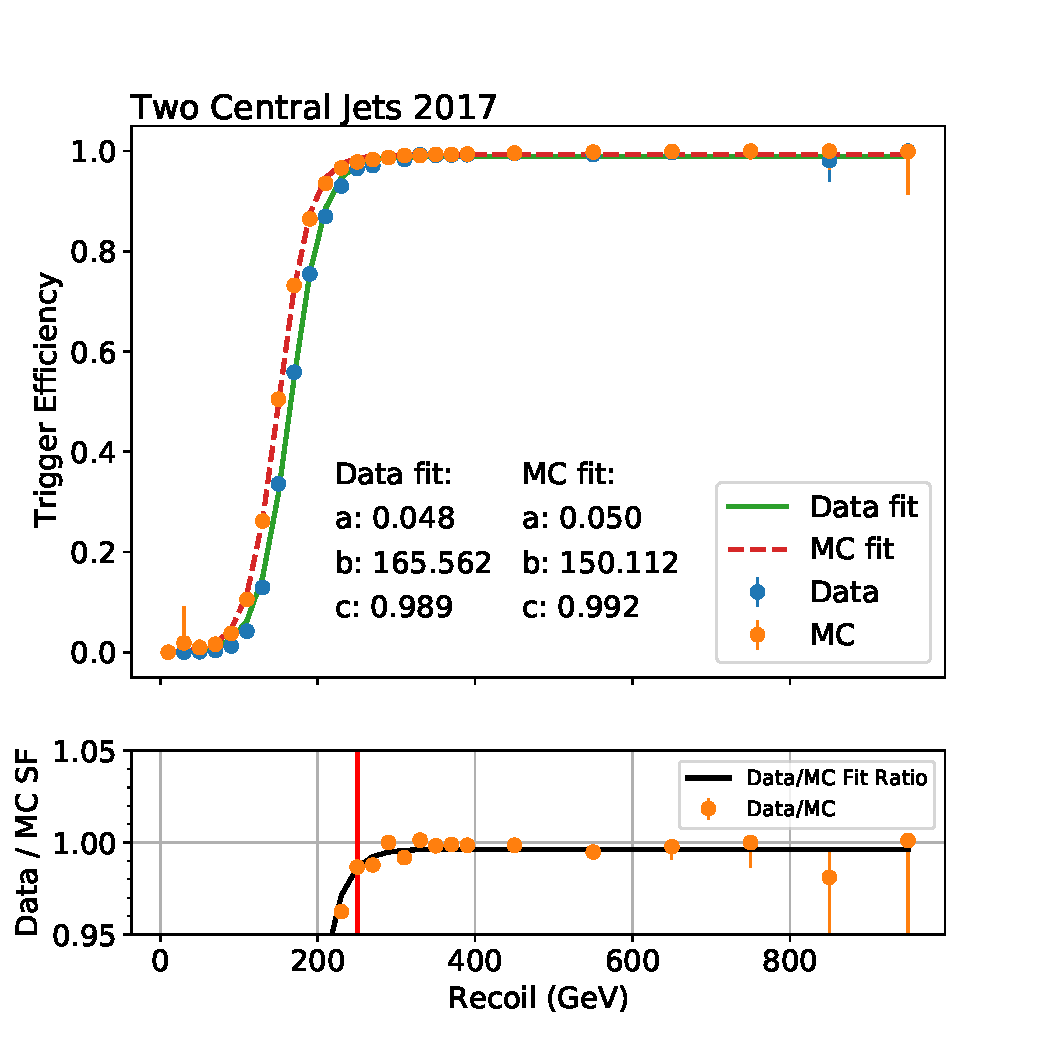
\includegraphics[width=0.49\textwidth]{Efficiency/METTrigger/eff_fit_two_central_jets_2017.pdf}
    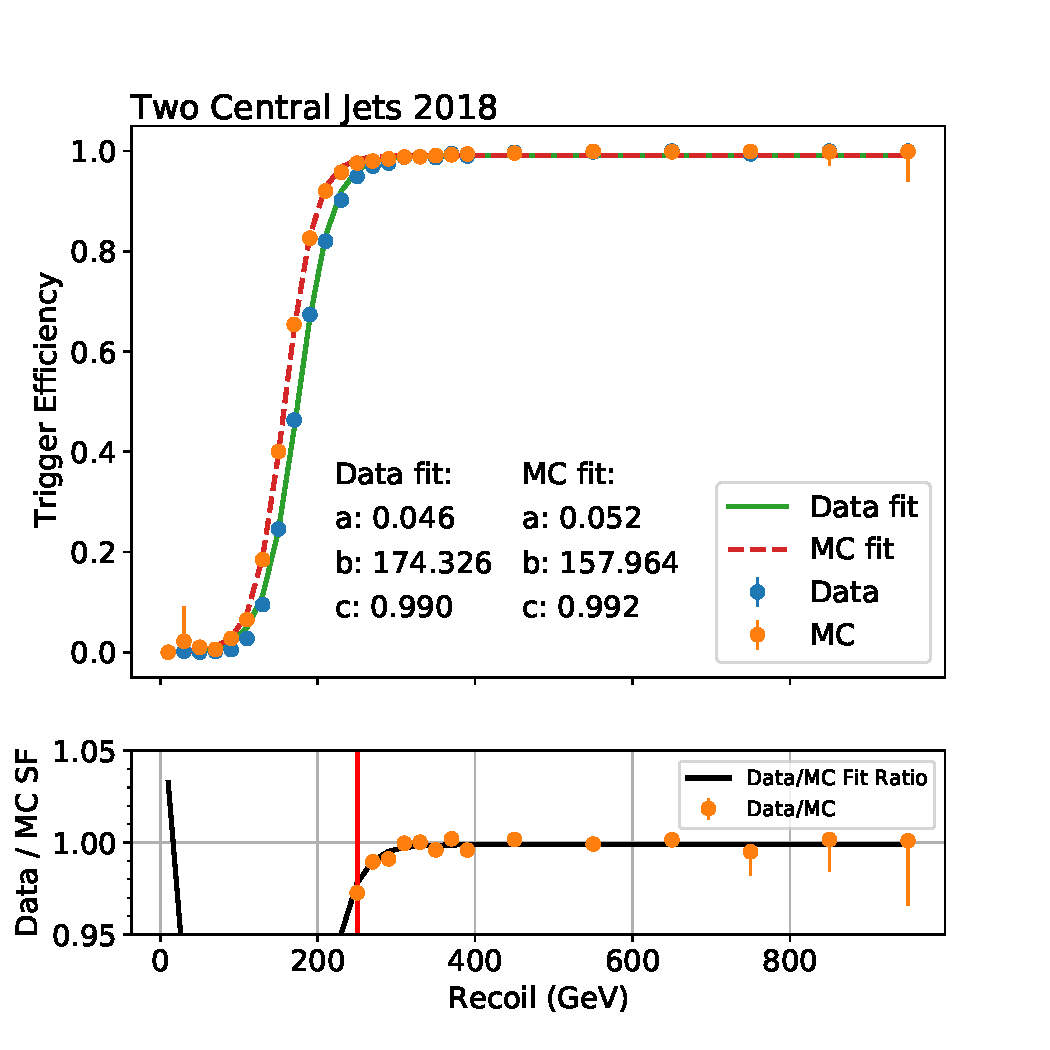
\includegraphics[width=0.49\textwidth]{Efficiency/METTrigger/eff_fit_two_central_jets_2018.pdf}
    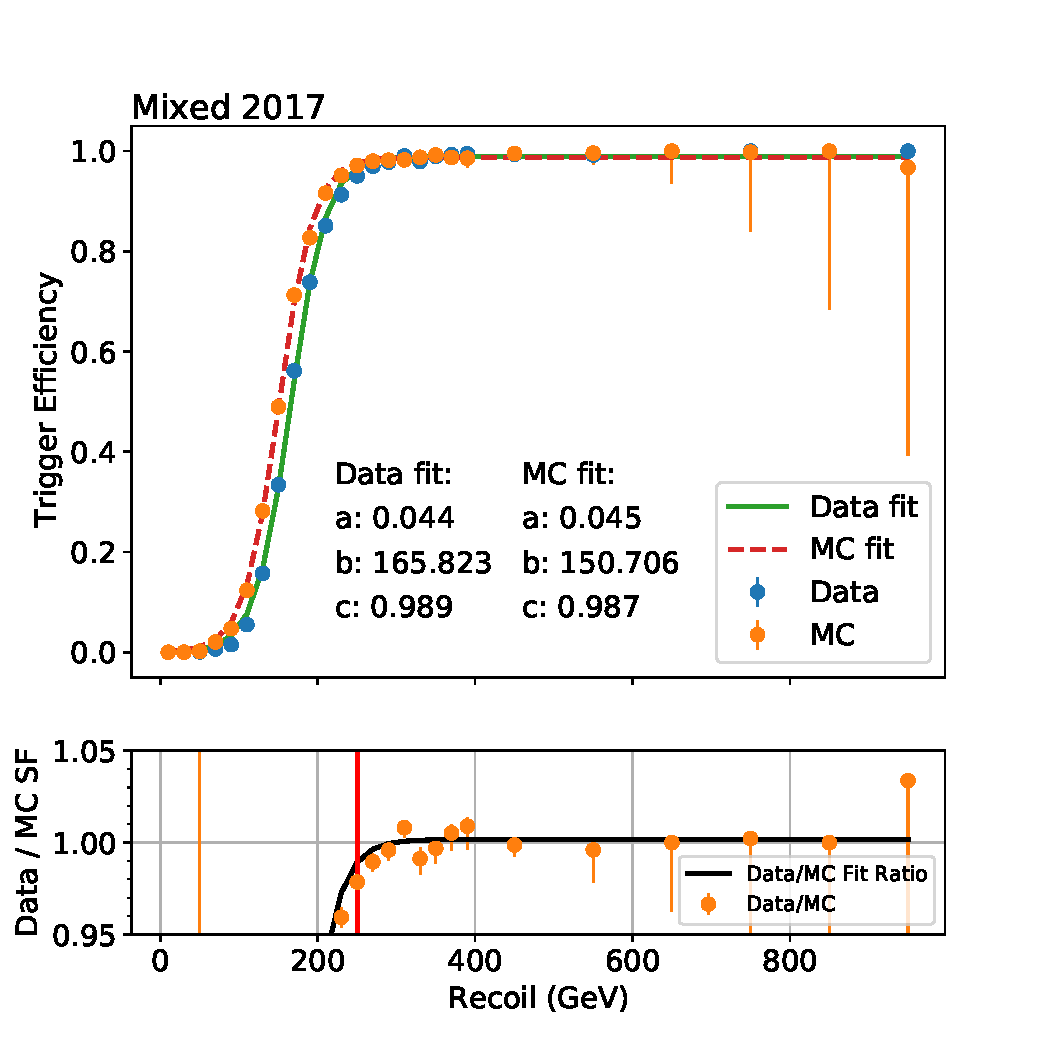
\includegraphics[width=0.49\textwidth]{Efficiency/METTrigger/eff_fit_one_jet_forward_one_jet_central_2017.pdf}
    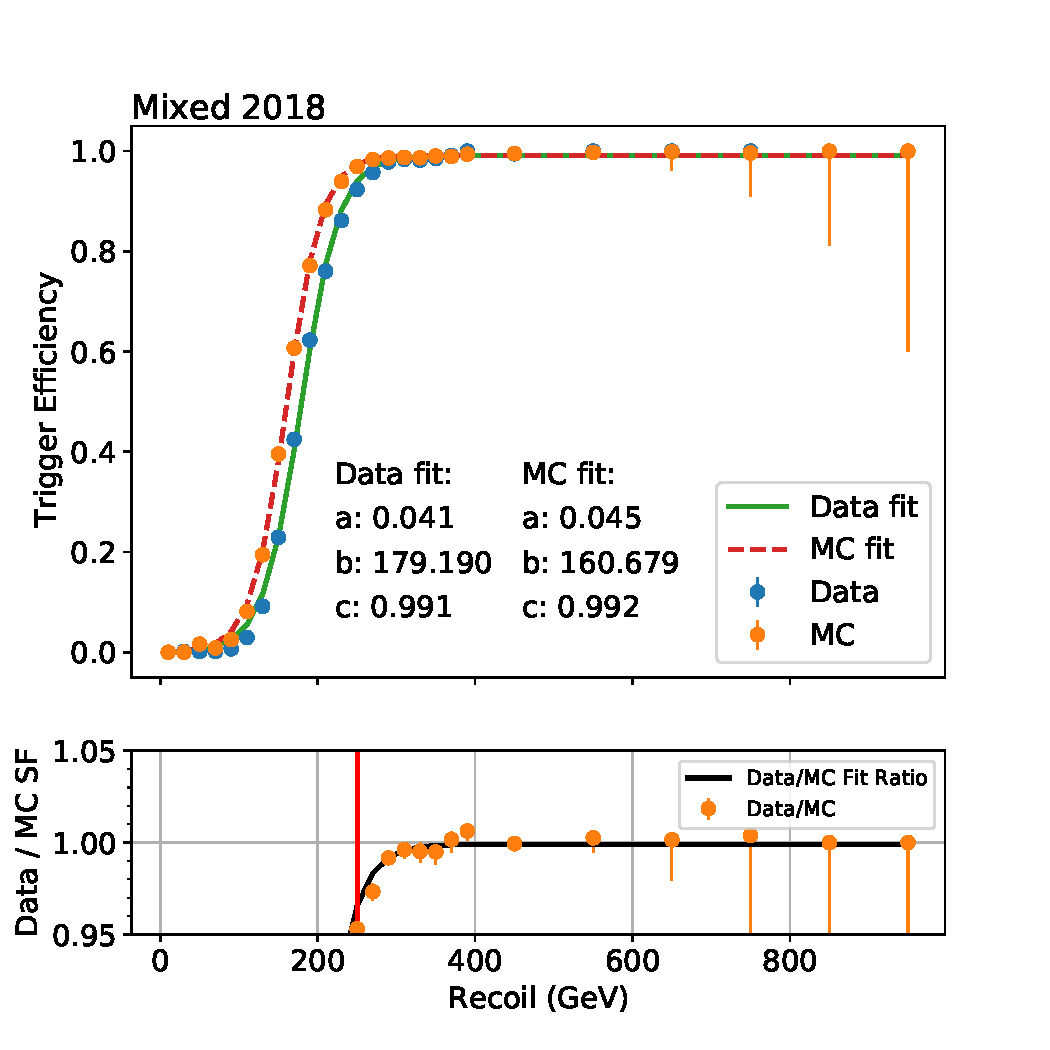
\includegraphics[width=0.49\textwidth]{Efficiency/METTrigger/eff_fit_one_jet_forward_one_jet_central_2018.pdf}
    \caption{MET trigger efficiencies for data and MC, for events where the two VBF jets are both central (top) 
    and where at least one jet is forward (bottom). Left column shows results with 2017 dataset, while the right column shows
    the results with 2018 dataset. To each efficiency curve, a sigmoid function 
    with three parameters are fitted: $f(x,a,b,c) = \frac{c}{1+e^{-a(x-b)}}$. 
    Resulting data/MC scale factors are shown in the bottom ratio pad for each case. The black line represents
    the ratio of two best-fit sigmoid functions, which is used as the correction factor to MC as a function of recoil.}
    \label{fig:sigmoid_fits_eff}
\end{figure}

\clearpage

\subsubsection{Photon trigger}
\label{subsubsec:photon_trig}

The photon trigger efficiency is measured using events collected with \texttt{HLT\_PFHT1050} 
trigger, which was fully unprescaled in 2017 and 2018, meaning that all the events passing the trigger were saved to the
disk.

Events are selected in the same way as for the photon control region in the analysis
(see Sec.~\ref{sec:selection_cr_g}) except for the photon $\pt$, recoil, $\HT$ and trigger requirements. To ensure an unbiased measurement, 
an offline $\HT$ of at least $1.5$ TeV is required, where $\HT$ is calculated as: 

\begin{equation}
  \HT = \sum_{jet} p_T^{jet}
  \label{eq:ht_def}
\end{equation}

In Eq.~\ref{eq:ht_def}, the sum runs over jets which pass the tight identification requirements 
and do not overlap with the selected photon within $\Delta R<0.4$. 
The trigger efficiency $\epsilon$ is then determined as:

$$\epsilon(\texttt{HLT\_Photon200}) = \frac{\text{Offline selection \&\& \texttt{HLT\_PFHT1050} \&\& 
\texttt{HLT\_Photon200}}}{\text{Offline selection \&\& \texttt{HLT\_PFHT1050}}} $$

The resulting efficiency in data and $\gamma +$jets \HT-binned simulation is shown in Fig.~\ref{fig:hlteff_photon}. In both data and simulation, 
the binned turn-on is fit using sigmoid functions, which are used to extract all further information. The trigger efficiencies in data and simulation are both 
found to be larger than $95\%$ for photon \pt values of more than $230$ GeV, which is used for the tight-identification requirement for photons reconstructed offline
(see Sec.~\ref{subsec:photons}). The MC-to-data scale factor is 
evaluated as the ratio of the sigmoid functions in data and simulation and is found to be within $1\%$ of unity consistent within an uncertainty of 1\% 
with all individual points. In the analysis implementation, the scale factor is implemented as an event-by-event weight based on the ratio of the sigmoid functions.

\begin{figure*}[hbtp]
    \begin{center}
        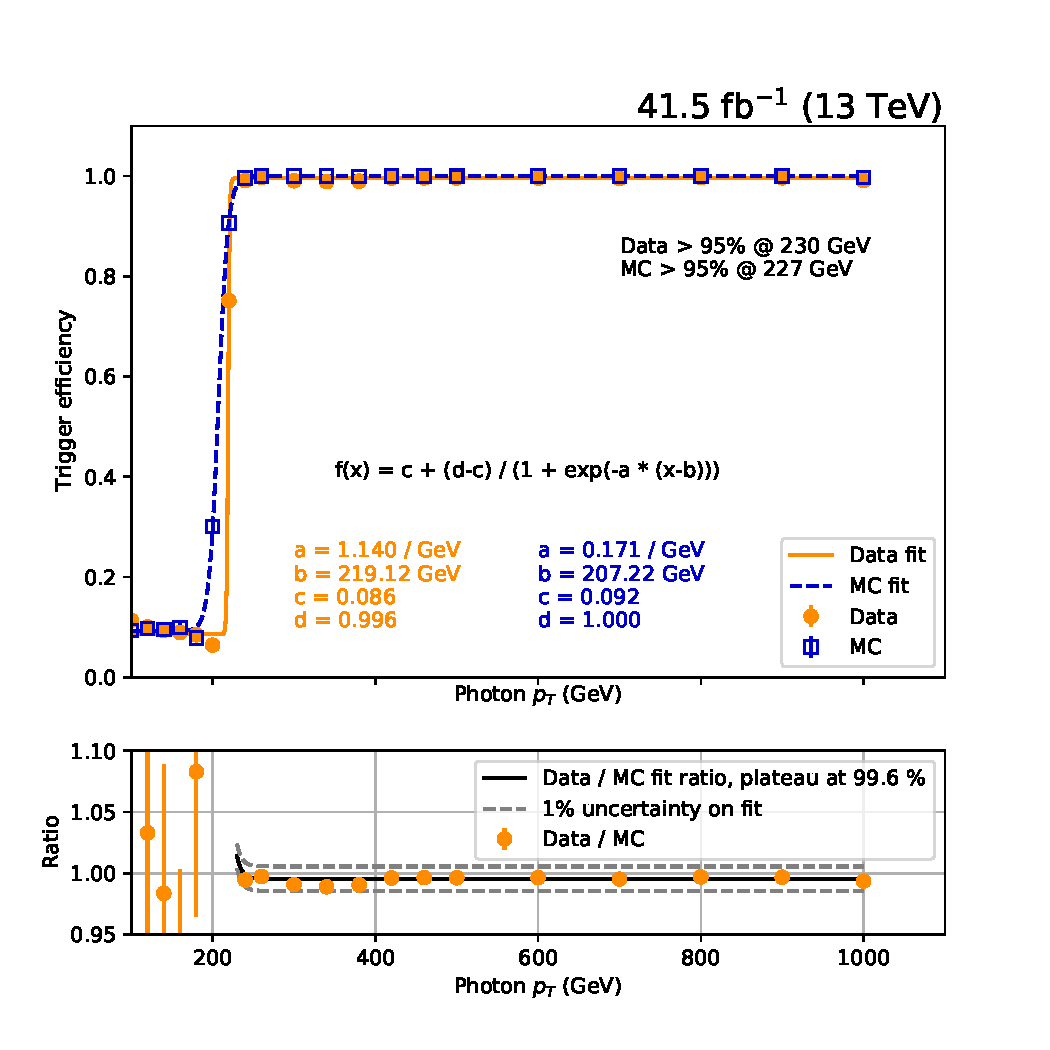
\includegraphics[width=0.6\textwidth]{Efficiency/Photon/fit_HLT_PFHT1050_2017.pdf}
        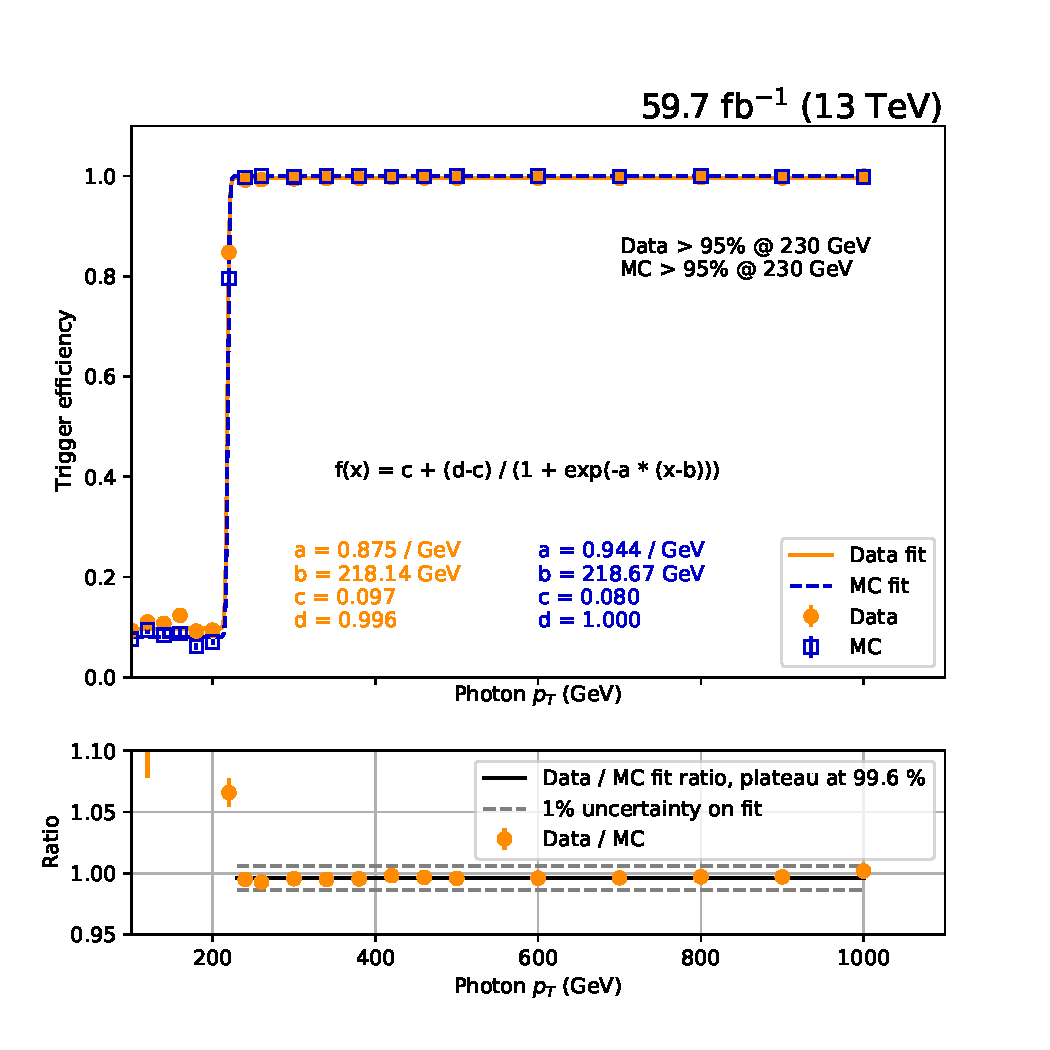
\includegraphics[width=0.6\textwidth]{Efficiency/Photon/fit_HLT_PFHT1050_2018.pdf}
        \caption{Efficiency of the \texttt{HLT\_Photon200} trigger in data and \HT-binned $\gamma+$jets MC for 2017 (top) and 2018 (bottom) 
        as a function of photon \pt. The orange and blue lines respectively represent sigmoid function fits to the turn-on in data and MC, 
        with the fit function and best-fit parameter values given in the respectively colored labels. The bottom panel shows the ratio of the values measured 
        in data over those in MC using orange markers. The solid black line corresponds to the ratio of the sigmoid fits to data and MC.}
        \label{fig:hlteff_photon}
    \end{center}
\end{figure*}

\clearpage

\subsubsection{Electron trigger}

This analysis uses the logical OR of three triggers for the selection of events with electrons in the final state:
\texttt{HLT\_Ele35*} (\texttt{HLT\_Ele32*}),
\texttt{HLT\_Ele115*} and \texttt{HLT\_Photon200} for 2017 (2018) data. The OR of these three triggers is henceforth referred to as ``the electron trigger'',
to simplify the discussion. The higher-threshold triggers are advantageous in that they either do not contain isolation requirements (\texttt{HLT\_Ele115}) or do not require 
a well-reconstructed track (\texttt{HLT\_Photon200}), both of which enhance the selection efficiency at large electron \pt.

The efficiency of the electron trigger is measured in data and simulation using a ``tag and probe'' method. Tag electrons are required to pass a 
logical OR of all triggers considered here. Both the tag electron and the probe electron are required to pass the tight identification criteria used for the analysis 
selection (see Tables~\ref{tab:tight_electron_def_barrel} and~\ref{tab:tight_electron_def_endcap}). In data, events are separated based on whether the probe electron passes 
the same trigger criteria as the tag. In both of these categories, 
separate fits to the distribution of the invariant mass of the tag-probe system are performed to extract the number of signal-like $Z(ee)$ events in each category, 
and the efficiency is defined as the ratio of the number of passing signal events and the number of all signal events. The efficiency in simulation is 
measured in a Drell-Yan sample, and the signal event counts are defined by simply counting all events in the passing and failing categories. The MC-to-data scale 
factor is then defined as the ratio of the efficiency in data and that in simulation. The efficiency in data, as well as the scale factors are shown in 
Fig.~\ref{fig:hlteff_electron}. Note the appearance of steps in the efficiency at electron momenta of $115$ and $200$ GeV, which are a result of the addition 
of the high-momentum triggers to the logical OR expression.

\begin{figure*}[hbtp]
    \begin{center}
    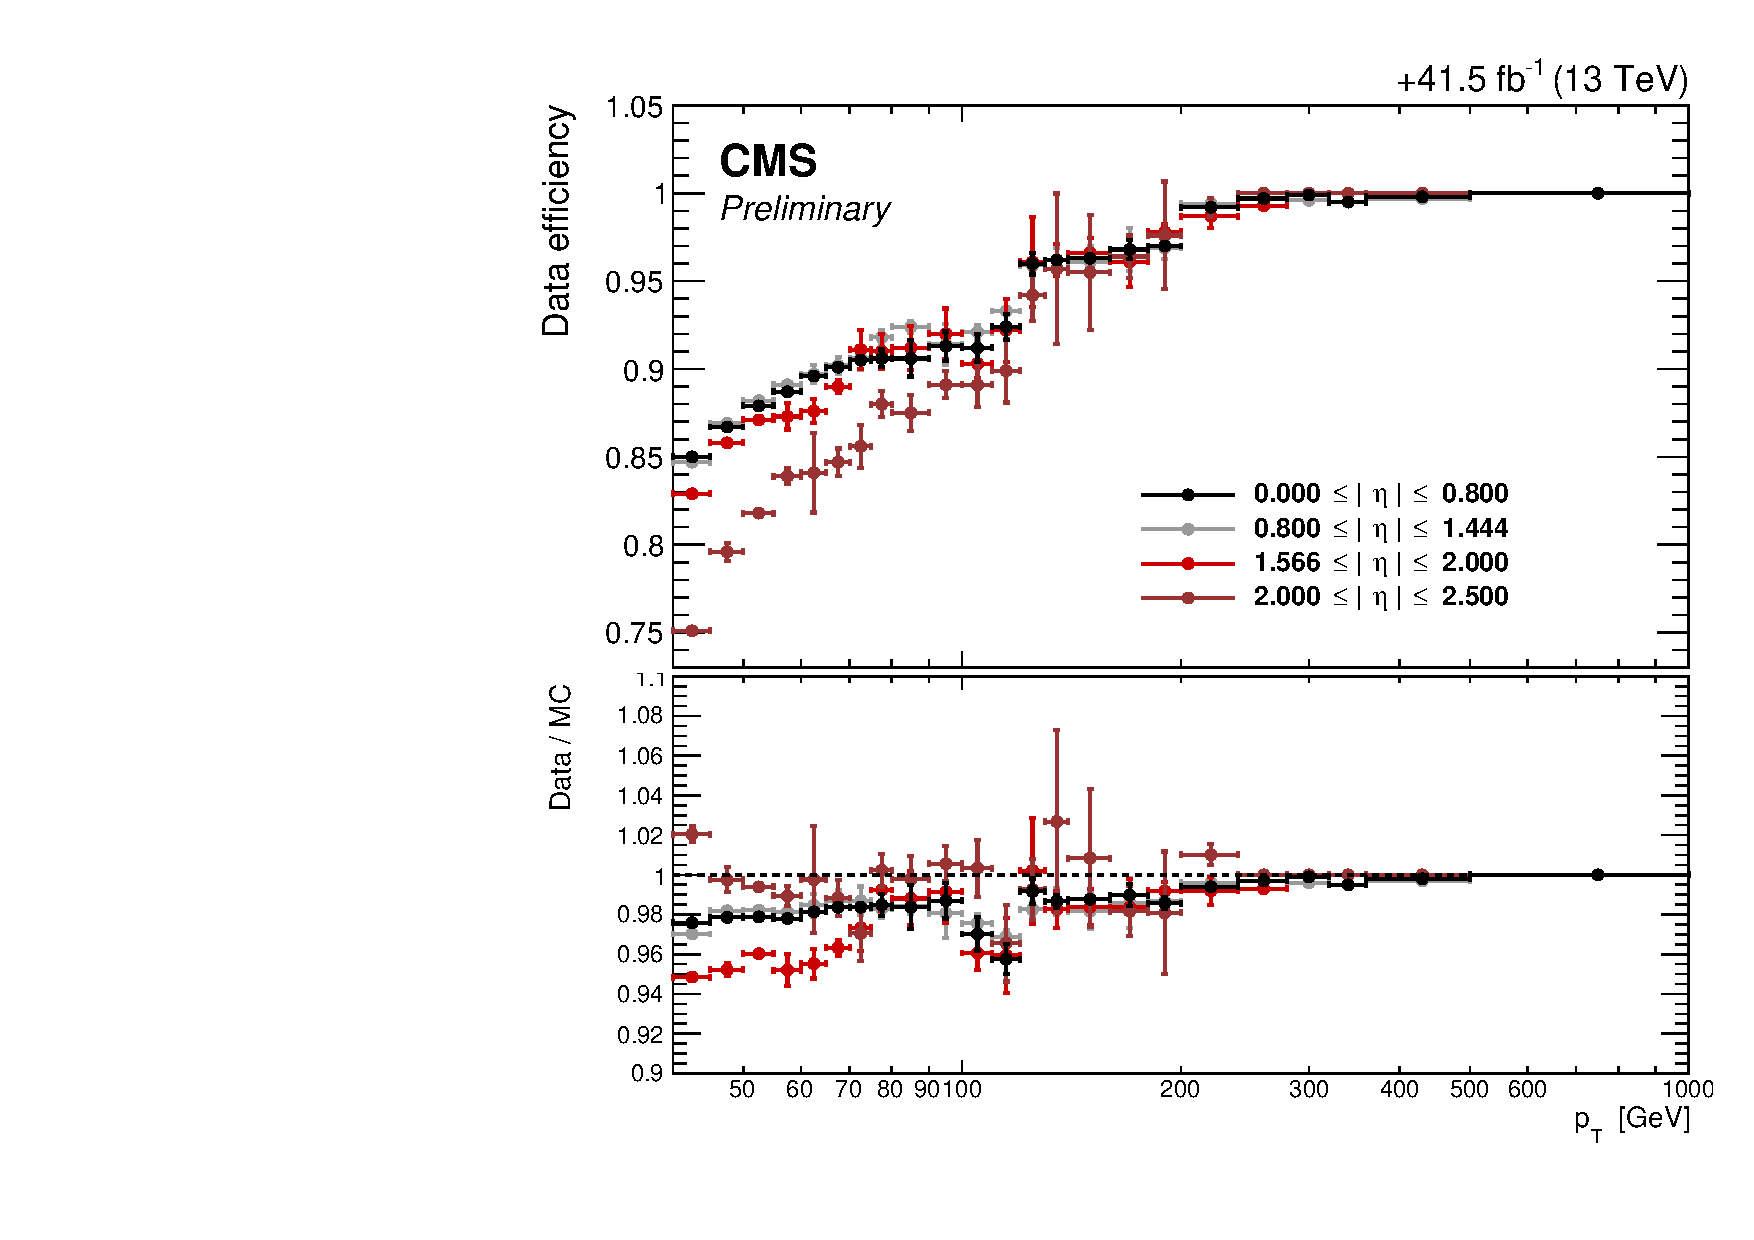
\includegraphics[width=0.6\textwidth]{Efficiency/Electron/electron_trig_eff_2017.pdf}
    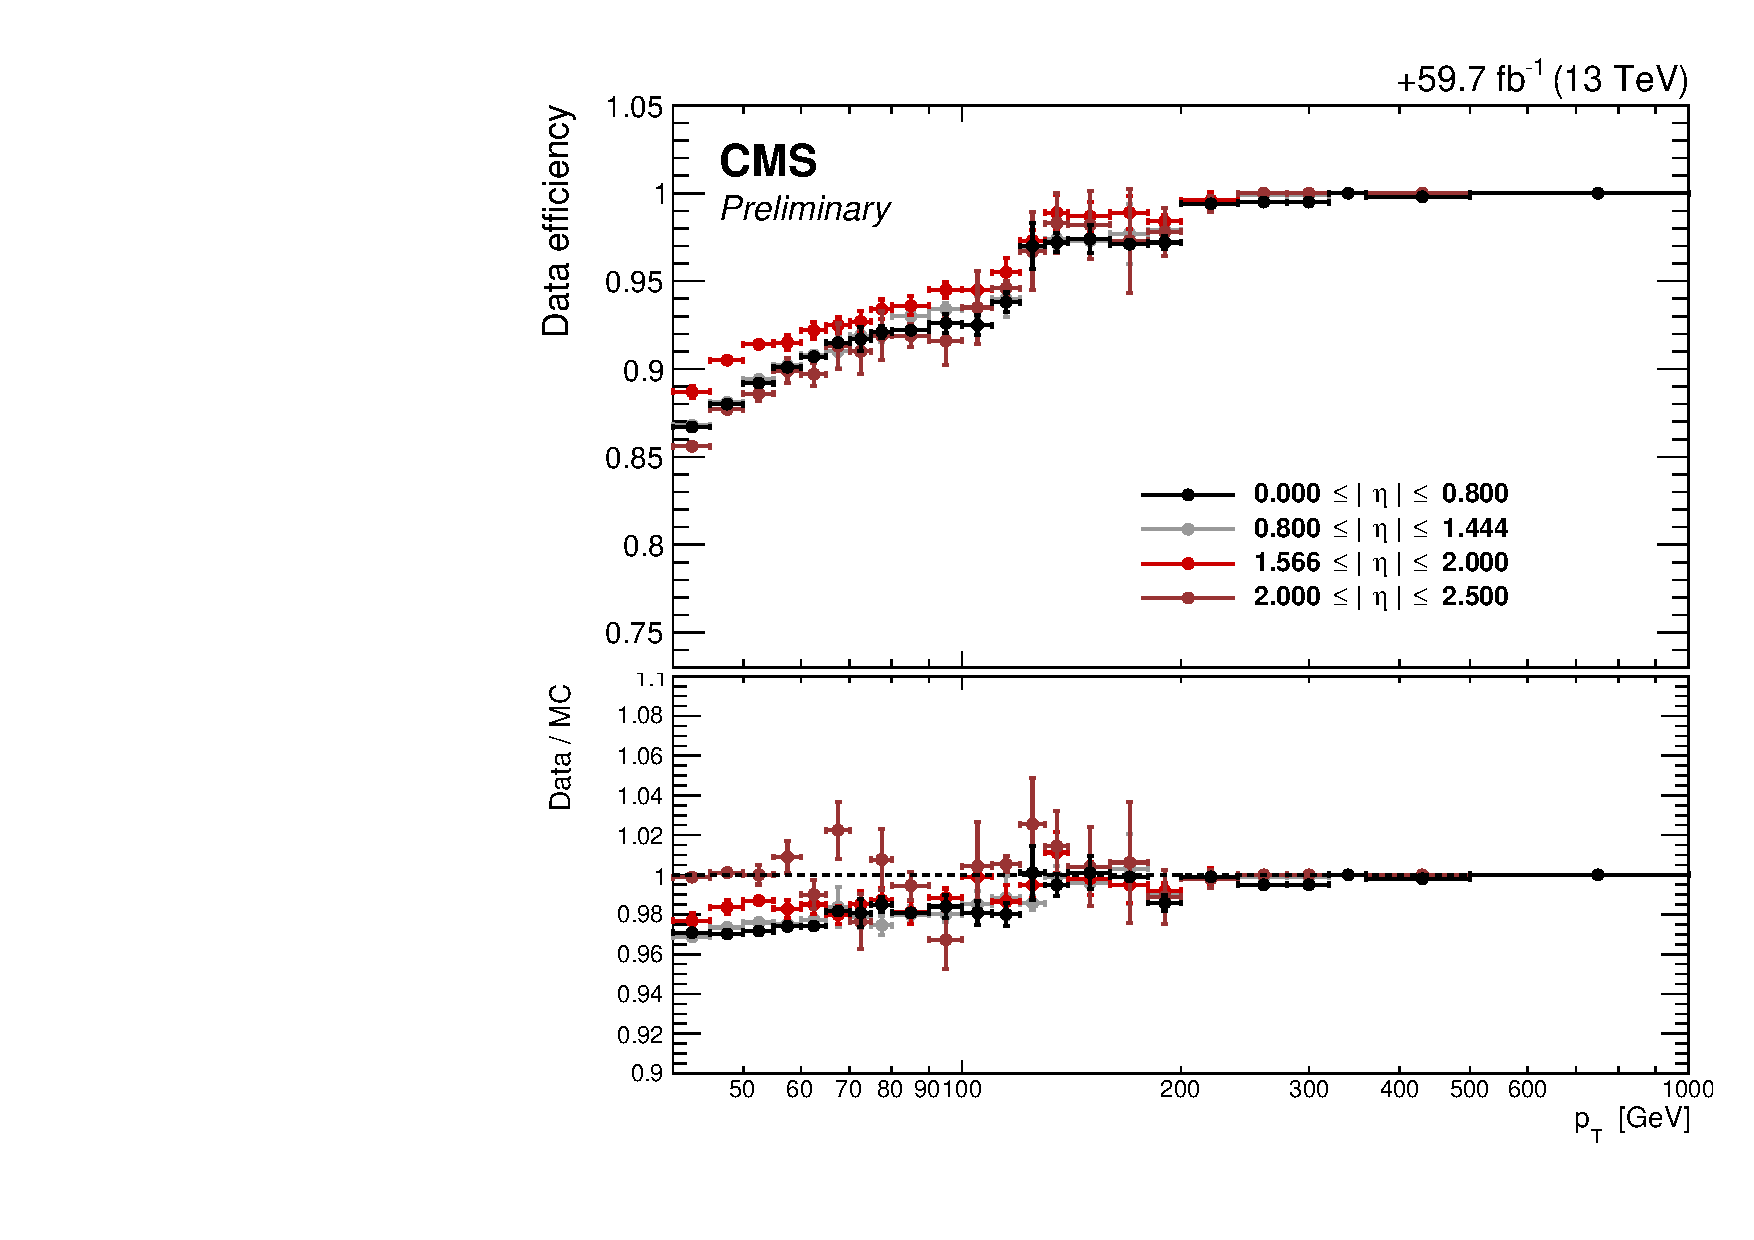
\includegraphics[width=0.6\textwidth]{Efficiency/Electron/electron_trig_eff_2018.pdf}
    \caption{Efficiency of the OR of the three triggers used to select electron events for 2017 (top) and 2018 (bottom) as a function of the electron 
        transverse momentum. The efficiency is shown for multiple regions of absolute electron pseudorapidity. In each plot, the upper panel shows 
        the efficiency in data, while the lower panel shows the ratio of the efficiency in data and that in simulation.}
    \label{fig:hlteff_electron}
    \end{center}
\end{figure*}

As shown in the bottom panel of Fig.~\ref{fig:hlteff_electron}, the data to MC scale factors are derived
from the two efficiency measurements from data and MC. Those correction factors are applied per-electron 
in the analysis to correct MC.

\subsection{Pileup reweighting}
\label{subsec:pu_reweighting}

The pileup (PU) conditions in the simulated samples are not identical to the ones observed in data, and a per-event reweighting is applied to remove the difference.
The reweighting is performed by matching the true pileup distribution of each simulated sample
with the pileup distribution in data. The pileup distribution in data is obtained through 
the pileupCalc tool, assuming a minimum bias cross section of 69.2$\pm 4.6\%$~mb, following the recommendations in \cite{pileup_twiki}.
The true pileup distributions in data and simulation are shown in Fig.~\ref{fig:purwg_true}, which show the normalized number of events as a function of 
the number of reconstructed collision vertices. 
The distribution of the number of reconstructed vertices 
for $W\to \mu\nu$ events before and after PU reweighting is shown in Fig.~\ref{fig:purwt_npv}. The distribution of the event energy density 
$\rho$ is shown in Fig.~\ref{fig:purwt_rho}, again before and after PU reweighting. 
In terms of these two variables, it is observed that PU reweighting improves the agreement between data and MC.

\begin{figure}[ht!]
  \begin{center}
    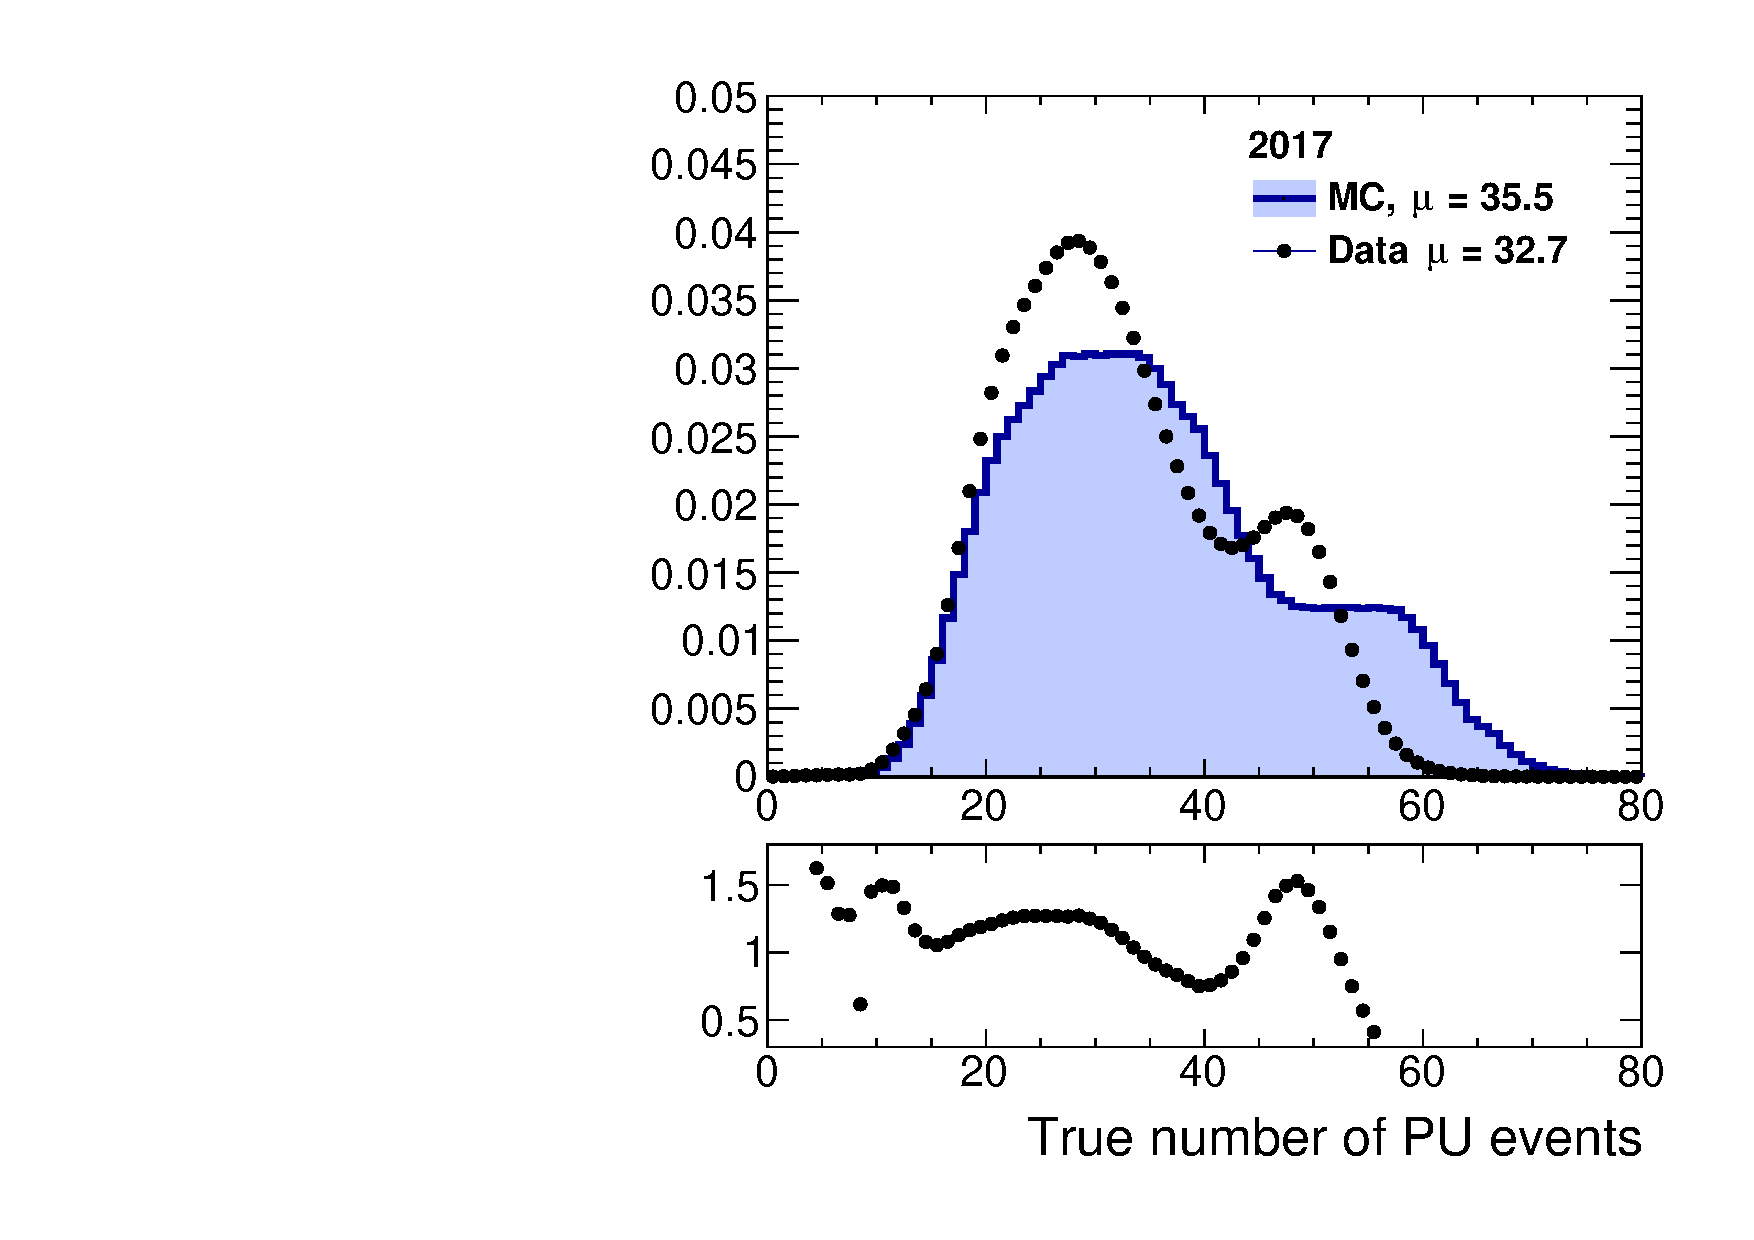
\includegraphics[width=0.49\textwidth]{Pileup/pu_weights_2017.pdf}
    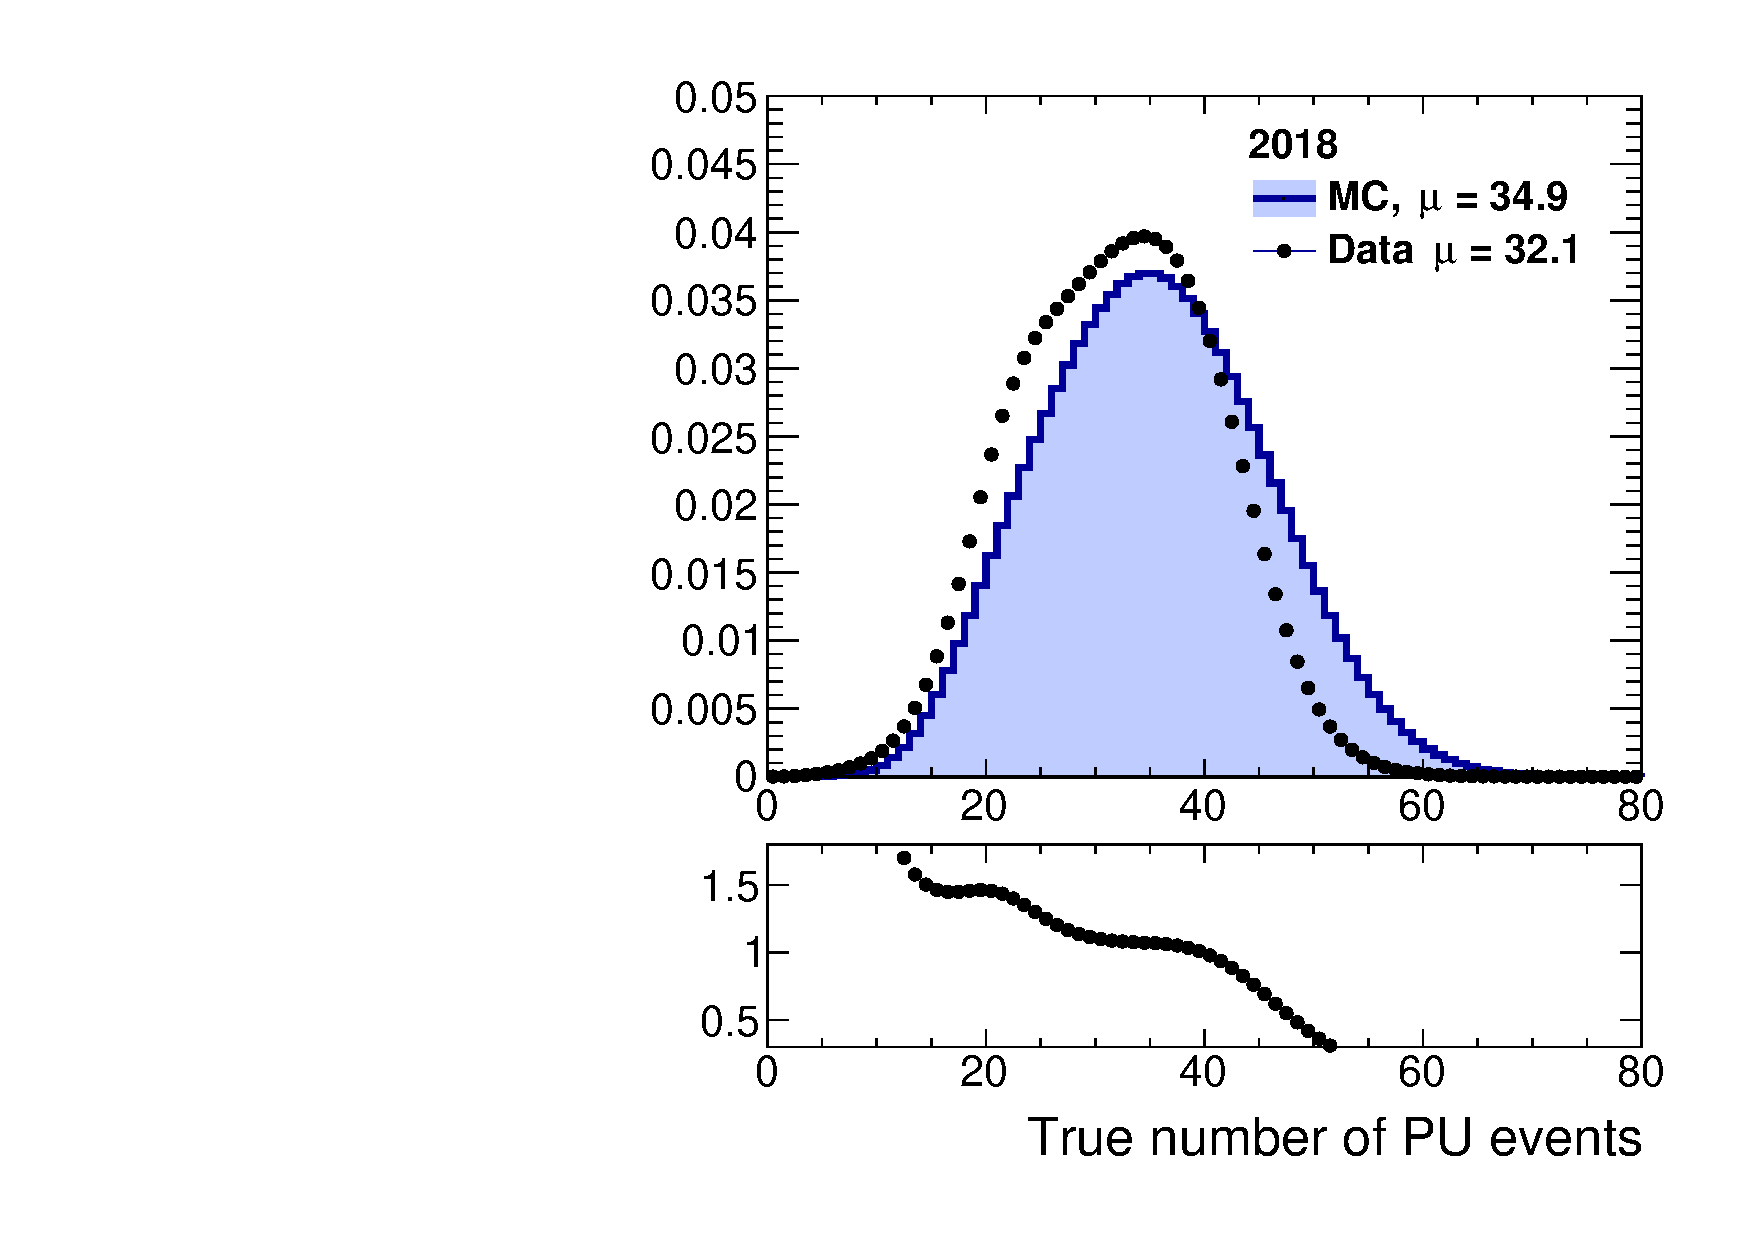
\includegraphics[width=0.49\textwidth]{Pileup/pu_weights_2018.pdf}
    \caption{
        Distribution of the true number of PU events in data and simulation for 2017 (left) and 2018 (right).
        The distributions for data are extracted assuming a minimum bias cross section of $69.2~\mathrm{mb}$.
    }
    \label{fig:purwg_true}
  \end{center}
\end{figure}

\begin{figure}[ht!]
  \begin{center}
    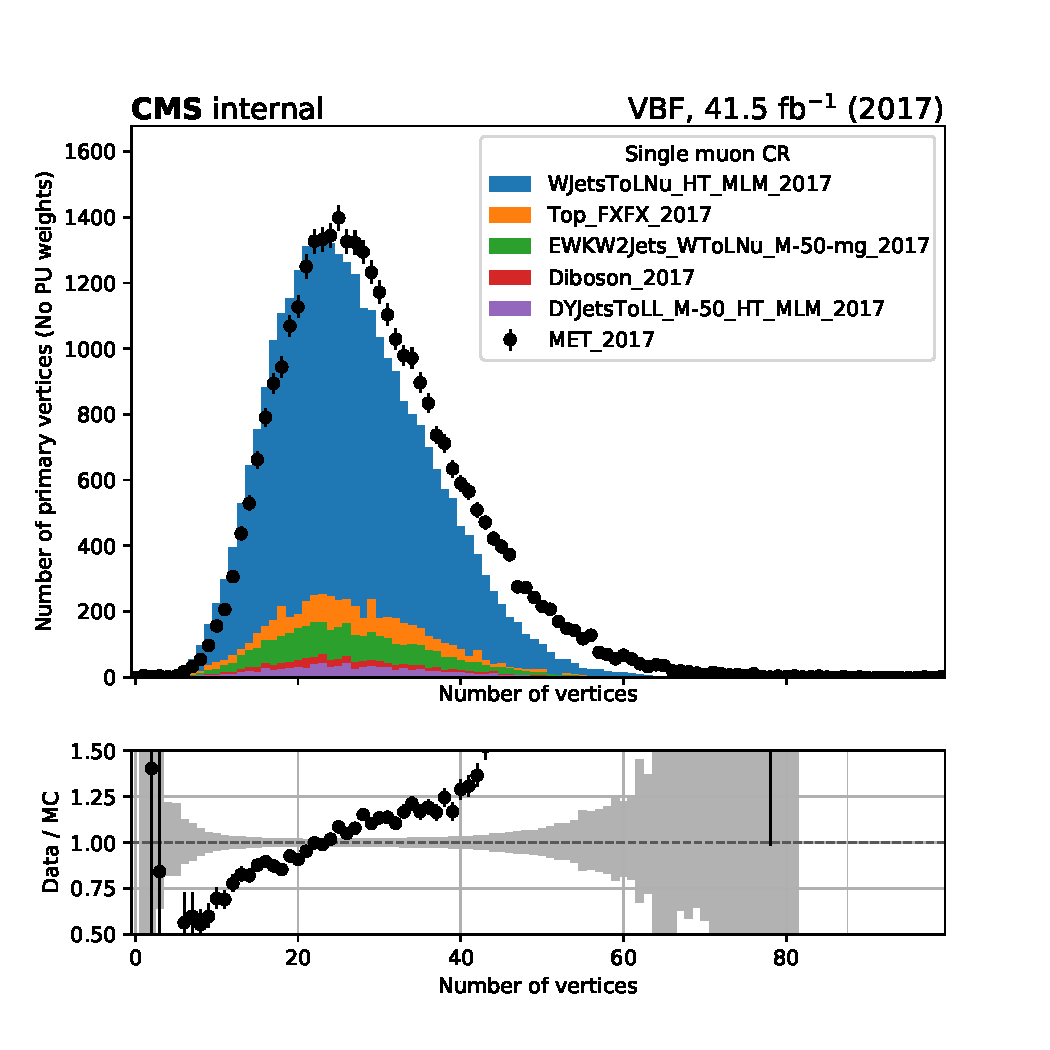
\includegraphics[width=0.49\textwidth]{Pileup/cr_1m_vbf_npv_nopu_2017.pdf}
    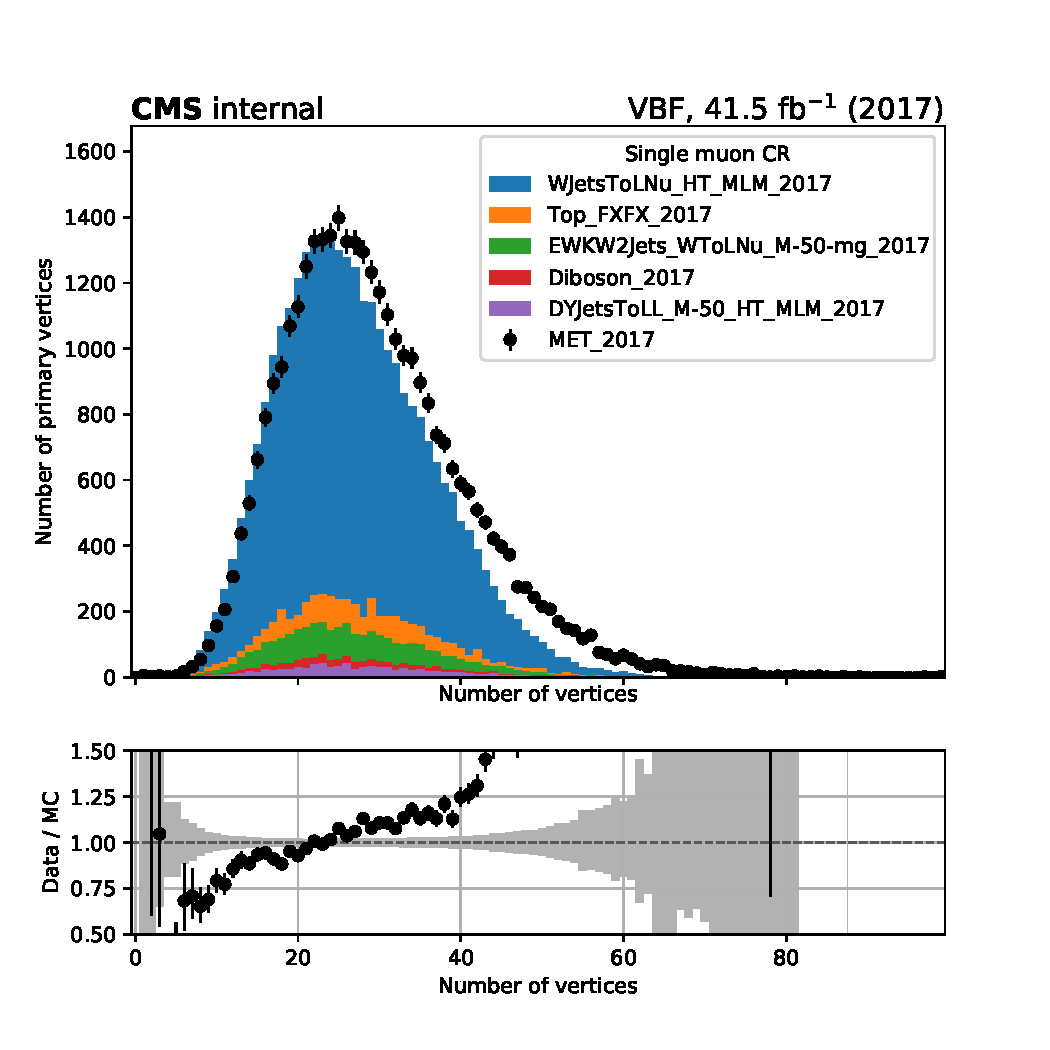
\includegraphics[width=0.49\textwidth]{Pileup/cr_1m_vbf_npv_2017.pdf}
    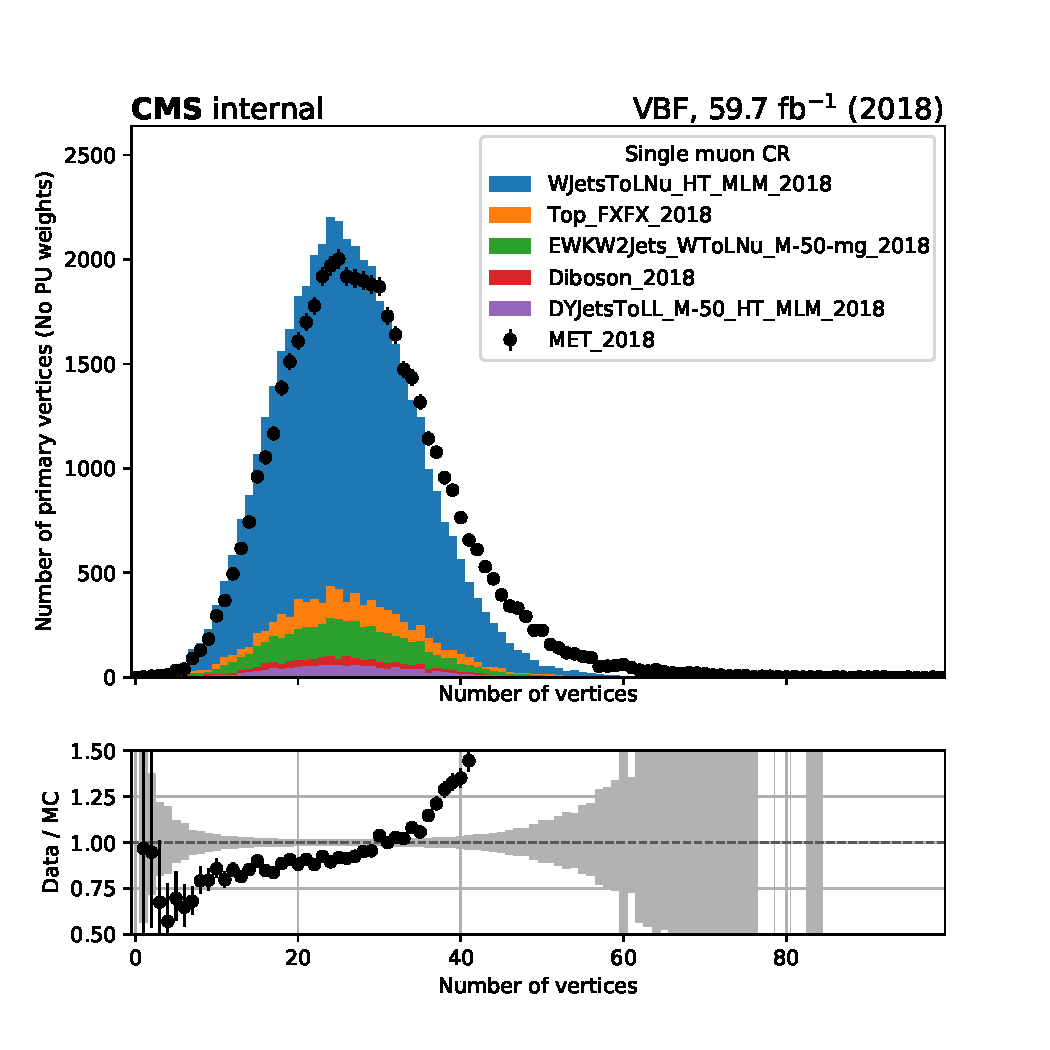
\includegraphics[width=0.49\textwidth]{Pileup/cr_1m_vbf_npv_nopu_2018.pdf}
    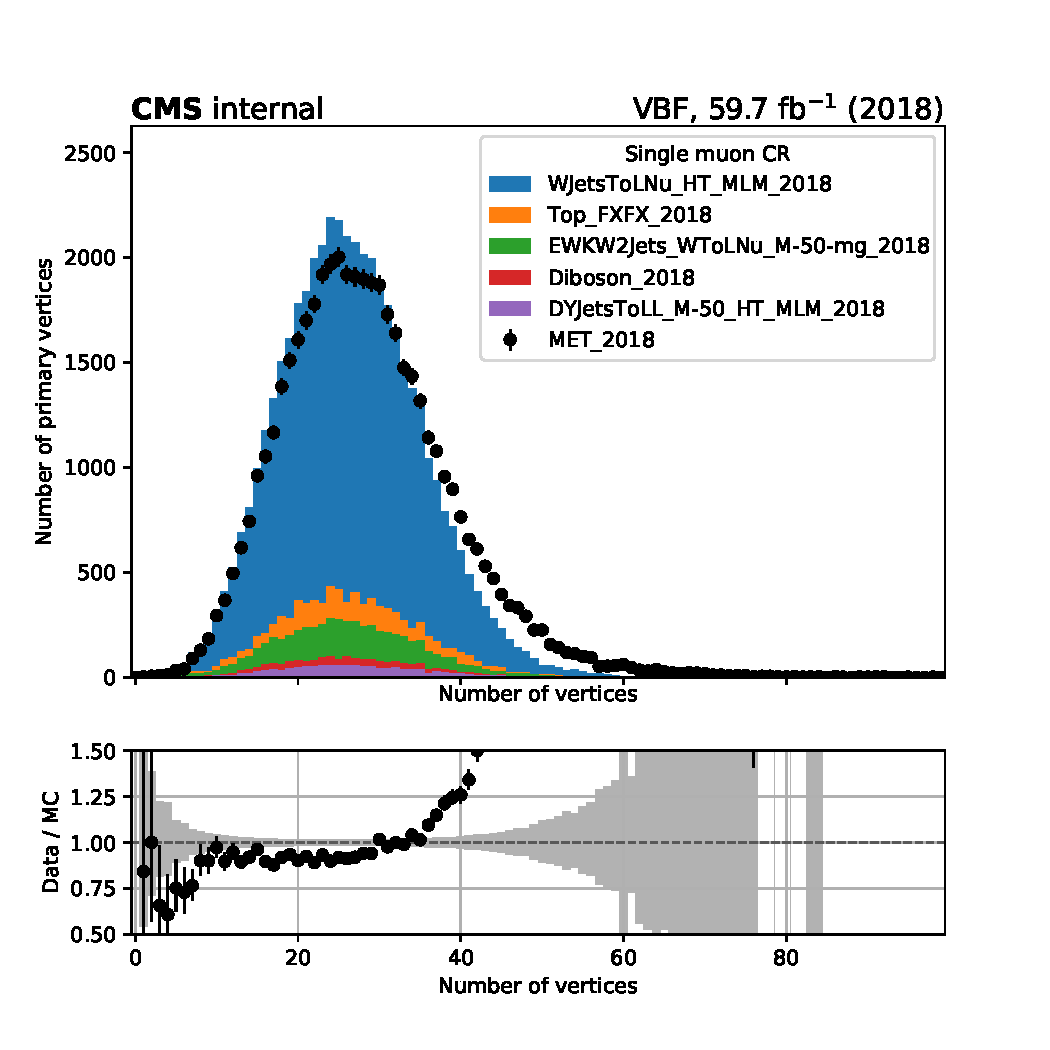
\includegraphics[width=0.49\textwidth]{Pileup/cr_1m_vbf_npv_2018.pdf}
    \caption{
        Distribution of the number of vertices in \Wmn~events in data and
        simulation before pileup re-weighting (left) and after pileup reweighting (right).
        The Monte Carlo is normalized to the luminosity of 41.53 and 59.7 fb$^{-1}$, respectively for 2017 and 2018.
    }
    \label{fig:purwt_npv}
  \end{center}
\end{figure}

\begin{figure}[ht!]
  \begin{center}
    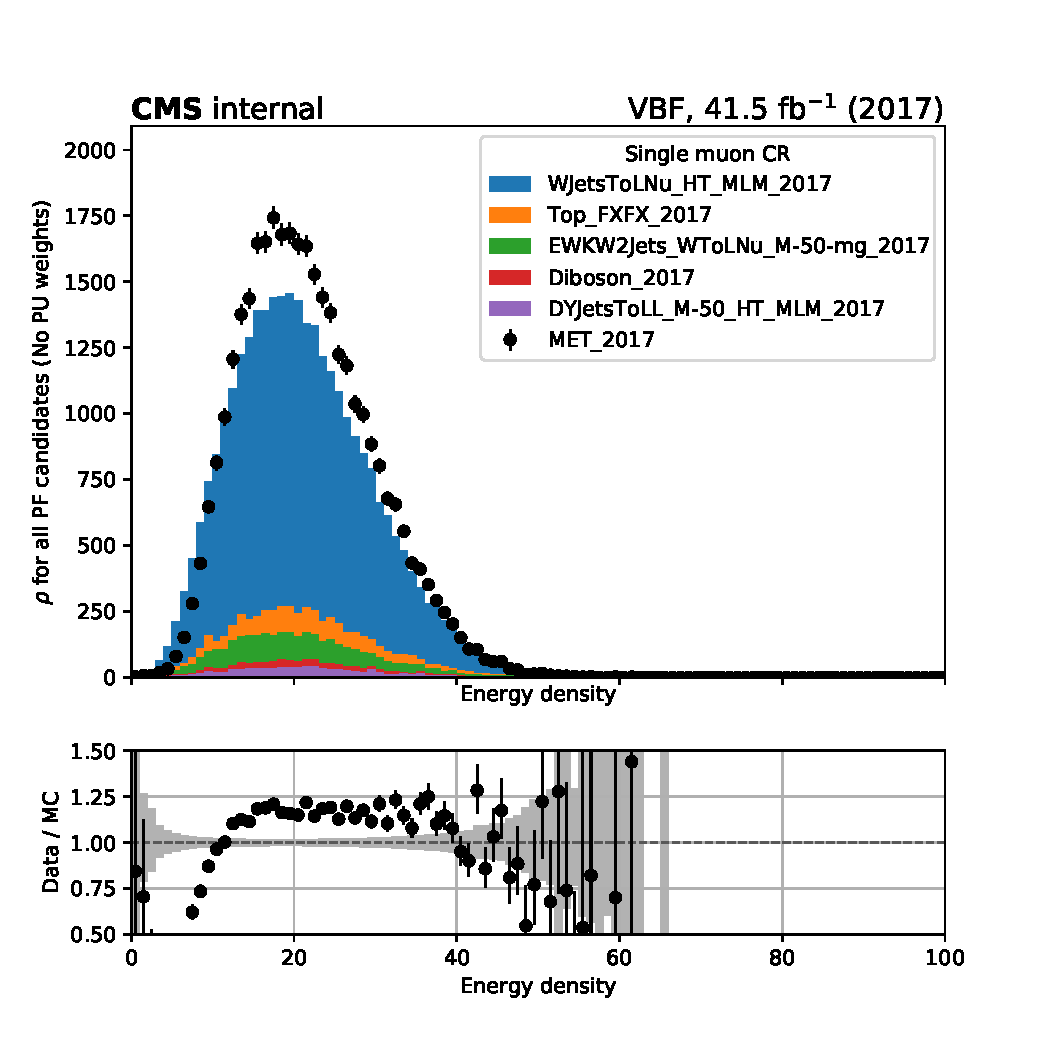
\includegraphics[width=0.49\textwidth]{Pileup/cr_1m_vbf_rho_all_nopu_2017.pdf}
    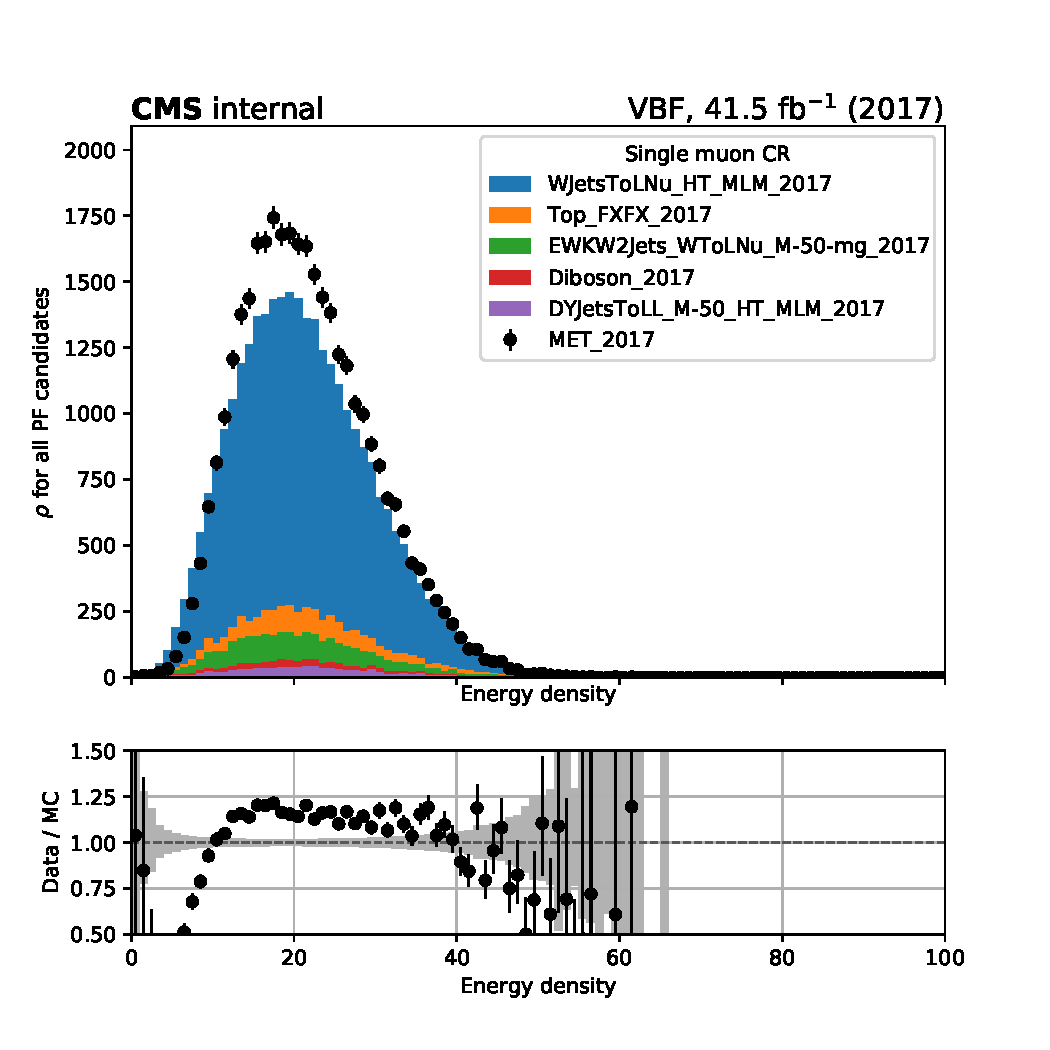
\includegraphics[width=0.49\textwidth]{Pileup/cr_1m_vbf_rho_all_2017.pdf}
    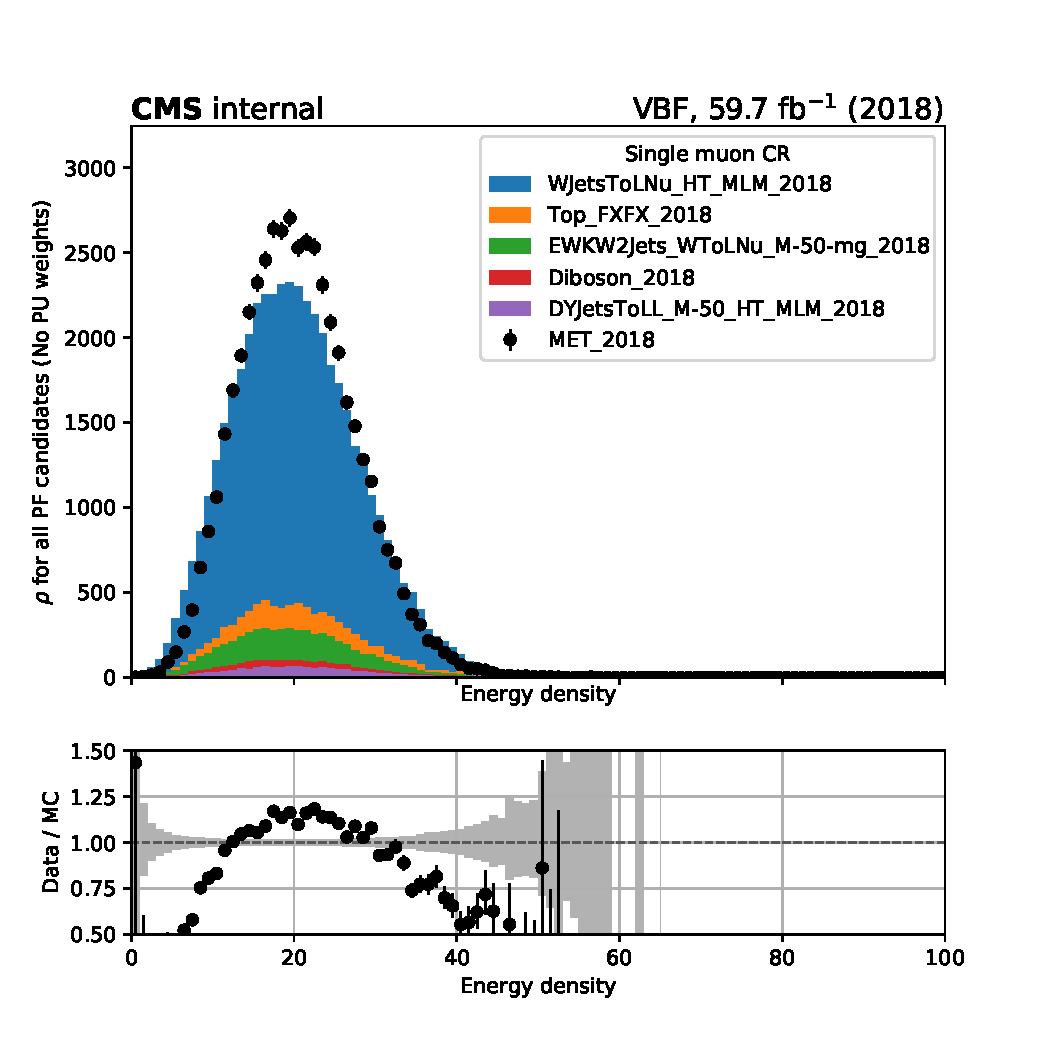
\includegraphics[width=0.49\textwidth]{Pileup/cr_1m_vbf_rho_all_nopu_2018.pdf}
    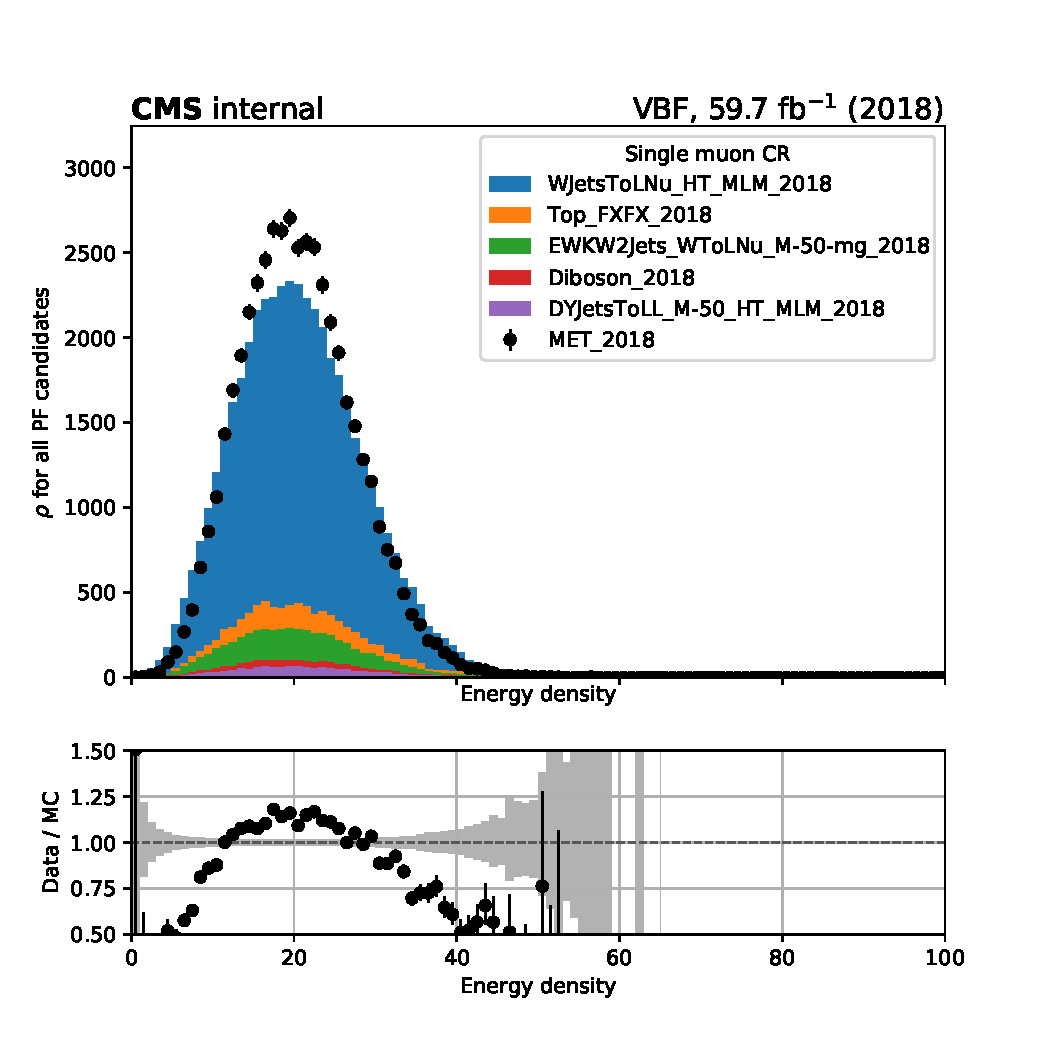
\includegraphics[width=0.49\textwidth]{Pileup/cr_1m_vbf_rho_all_2018.pdf}
    \caption{
        Distribution of the event energy density $\rho$ in \Wmn~events in data and
        simulation before pileup re-weighting (left) and after pileup reweighting (right).
        The Monte Carlo is normalized to the luminosity of 41.53 and 59.7 fb$^{-1}$, respectively for 2017 and 2018.
    }
    \label{fig:purwt_rho}
  \end{center}
\end{figure}

\clearpage

\subsection{Lepton identification efficiency reweighting}
\label{subsec:lepton_id_reweighting}

Data-to-MC scale factors are applied to events in the control regions to
account for differences in the reconstruction, identification and isolation of leptons
between data and MC. These data-to-MC scale factors are derived from the efficiencies that are measured for the electron and muon
selections in bins of $\pt$ and $\eta$ in both data and MC. The muon reconstruction and identification scale factors are
provided by the relevant POGs. Electron identification scale factors are measured using a tag-and-probe method, and the results are reviewed 
and approved by EGamma POG.

The reconstruction scale factors for electrons are shown in Fig.~\ref{fig:sf_electron_reco}. The corresponding identification scale factors for 
veto and tight electrons are shown in Fig.~\ref{fig:sf_electron_id}, and include the effect of the isolation efficiency. 

The identification scale factors for muons are shown in Fig.~\ref{fig:sf_muon_id}. Here, isolation scale factors are applied separately and are 
shown in Fig.~\ref{fig:sf_muon_iso}. The corresponding corrections for muons are deemed negligible~\cite{CMS-MUO-TWIKI-SF}.

\begin{figure}[ht!]
  \begin{center}
    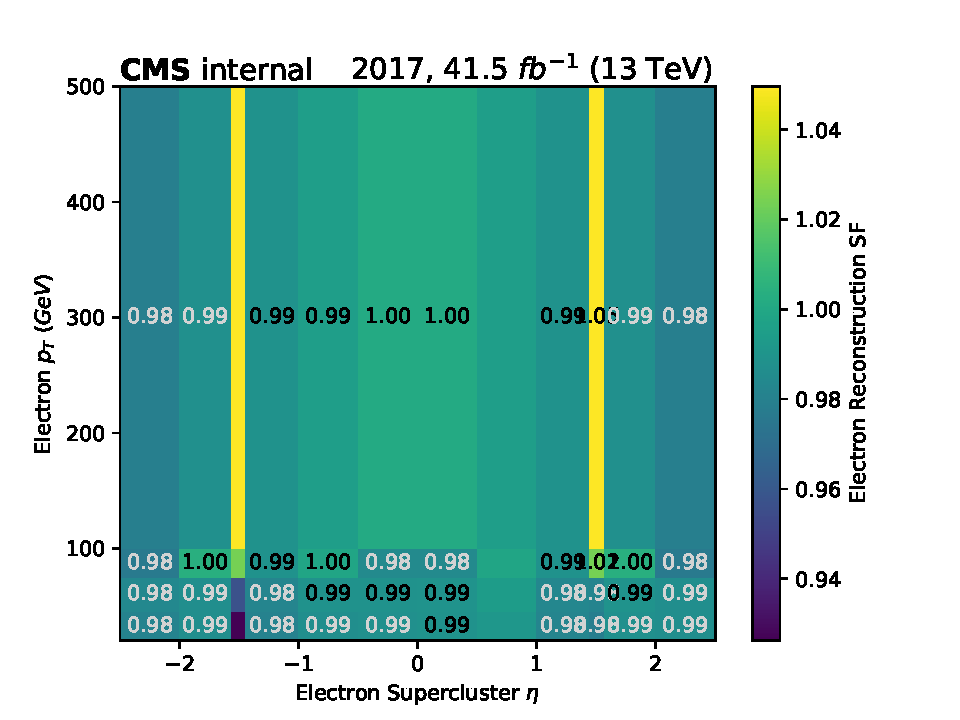
\includegraphics[width=0.49\textwidth]{ScaleFactors/Electron/electron_reco_2017.pdf}
    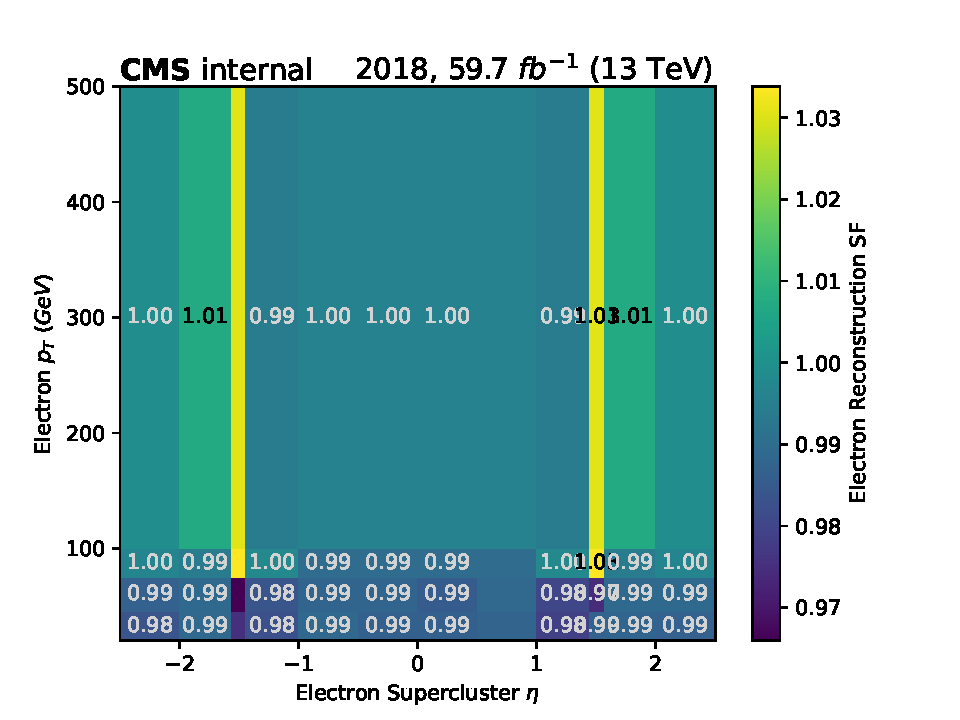
\includegraphics[width=0.49\textwidth]{ScaleFactors/Electron/electron_reco_2018.pdf} \\
    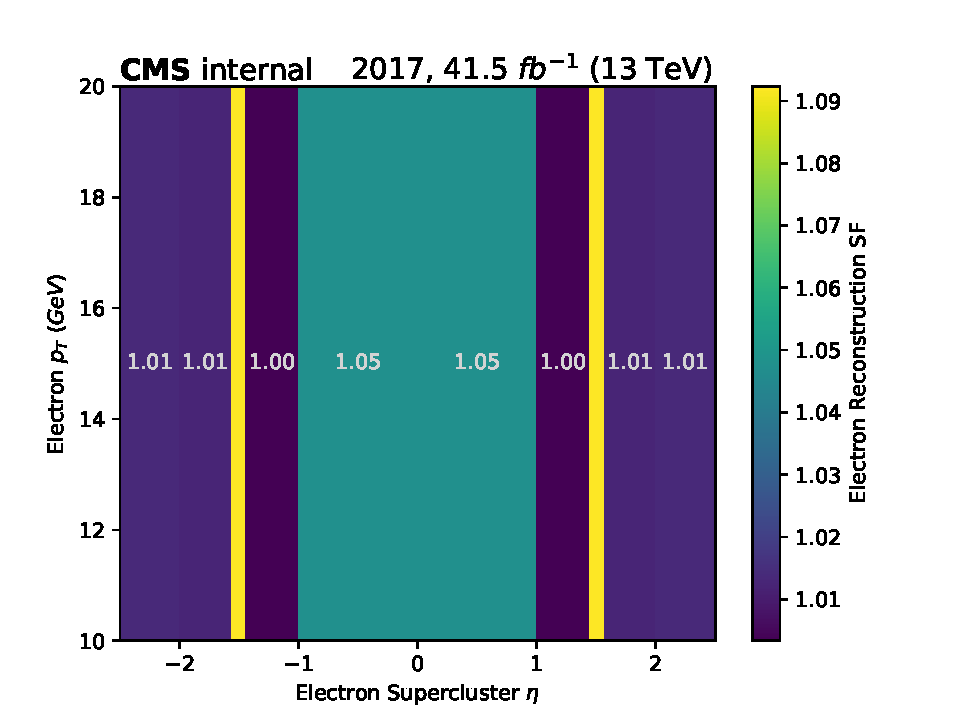
\includegraphics[width=0.49\textwidth]{ScaleFactors/Electron/electron_reco_ptbelow20_2017.pdf}
    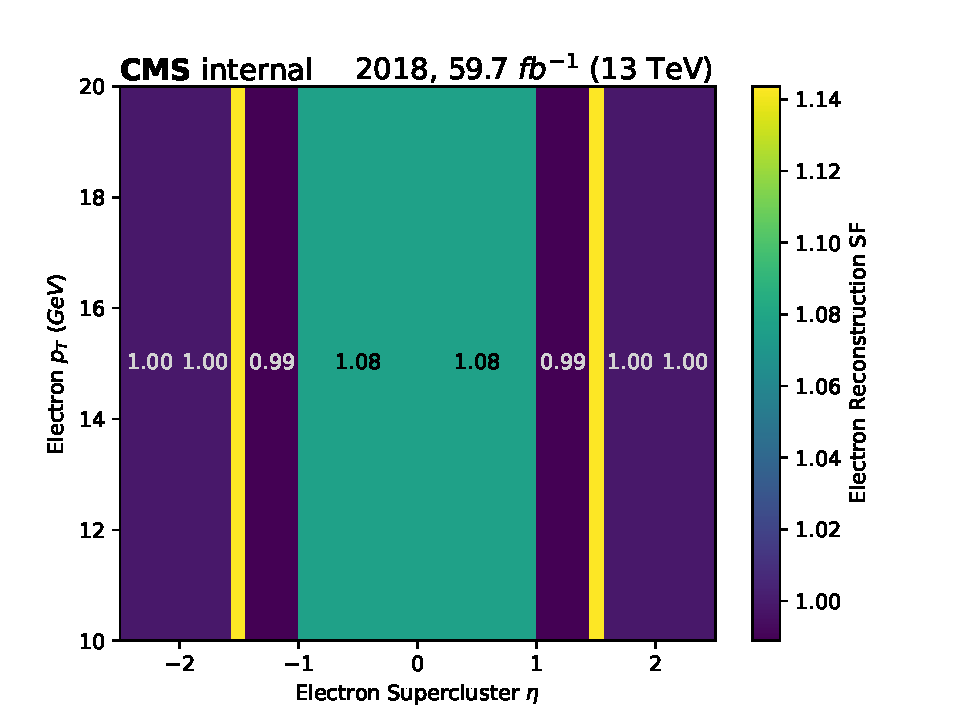
\includegraphics[width=0.49\textwidth]{ScaleFactors/Electron/electron_reco_ptbelow20_2018.pdf}

    \caption{
      Scale factors for the reconstruction efficiency of electrons starting from a super cluster for 2017 (left) and 2018 (right), for electrons with
      $\pt > 20 \ GeV$ (top) and $\pt < 20 \ GeV$ (bottom).
    }
    \label{fig:sf_electron_reco}
  \end{center}
\end{figure}

\begin{figure}[ht!]
  \begin{center}
    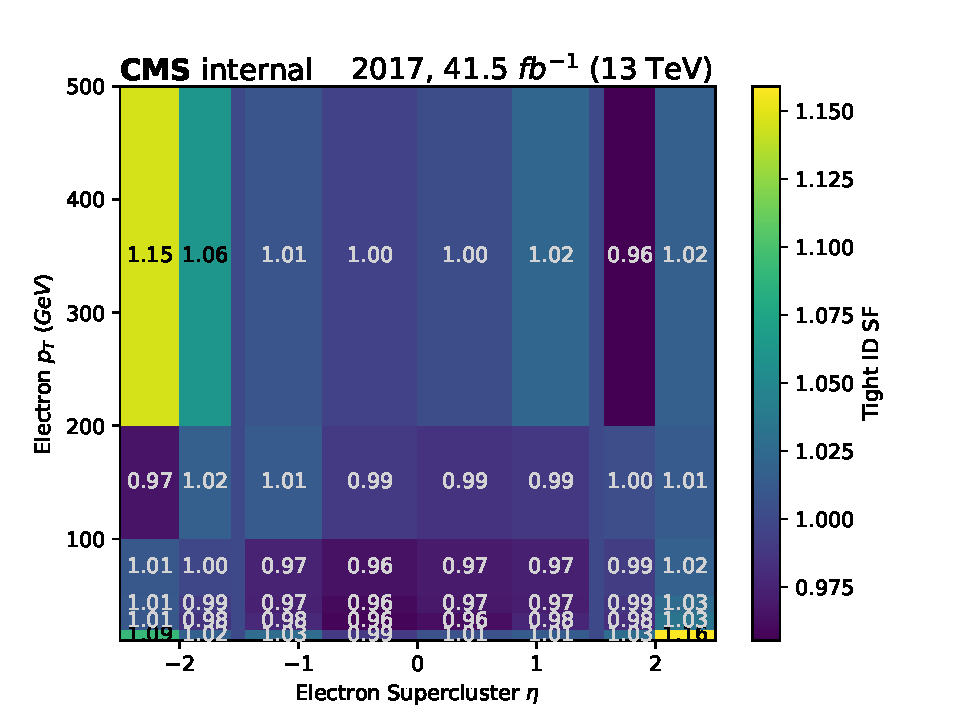
\includegraphics[width=0.45\textwidth]{ScaleFactors/Electron/electron_id_tight_2017.pdf}
    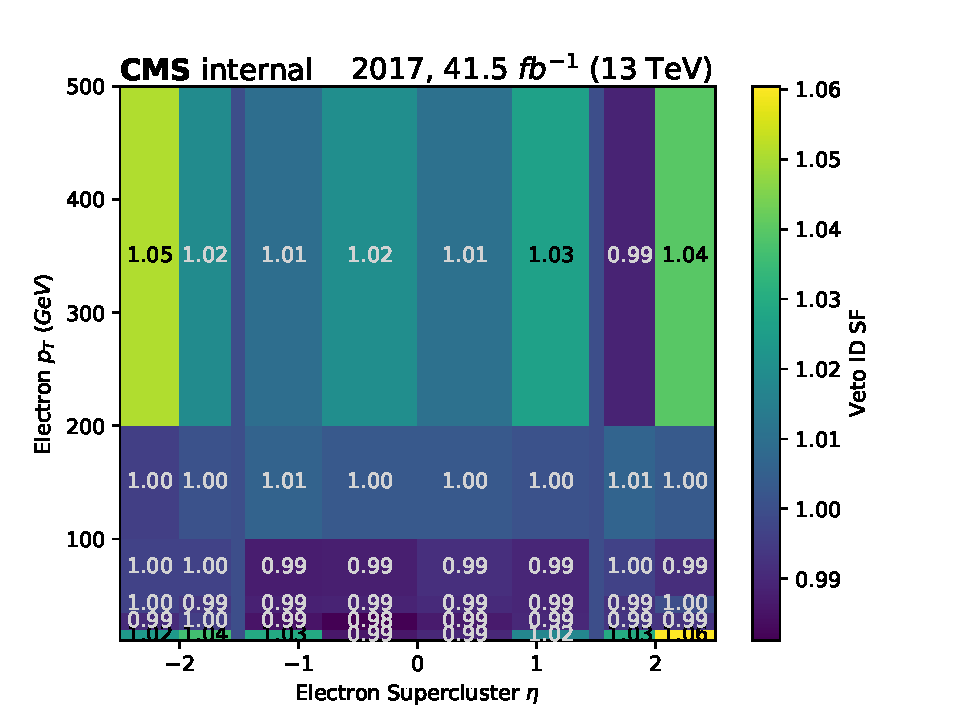
\includegraphics[width=0.45\textwidth]{ScaleFactors/Electron/electron_id_veto_2017.pdf} \\
    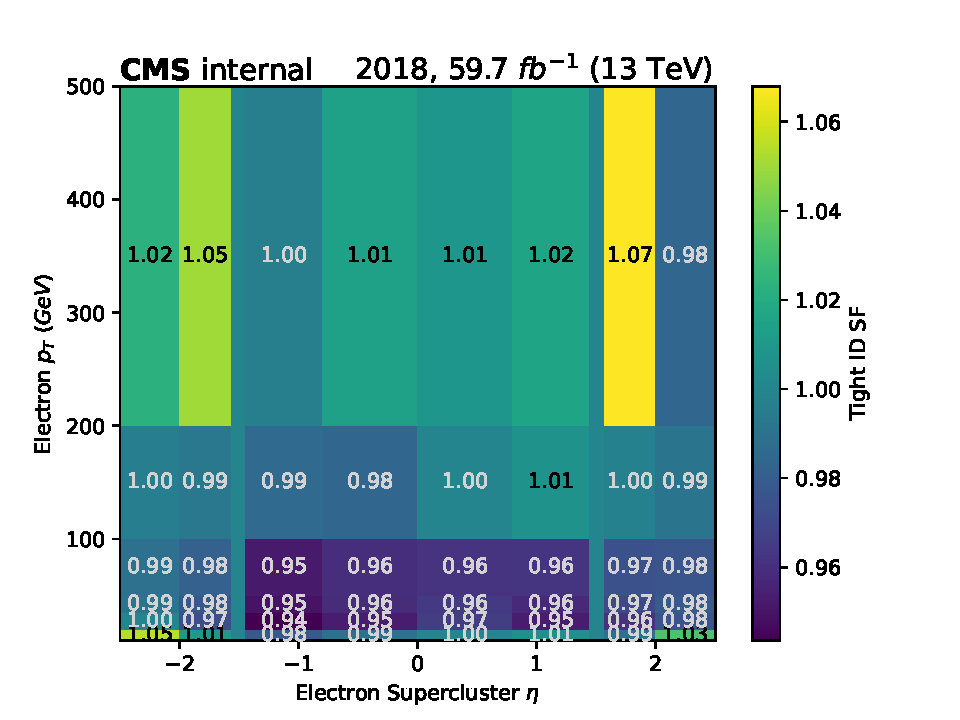
\includegraphics[width=0.45\textwidth]{ScaleFactors/Electron/electron_id_tight_2018.pdf}
    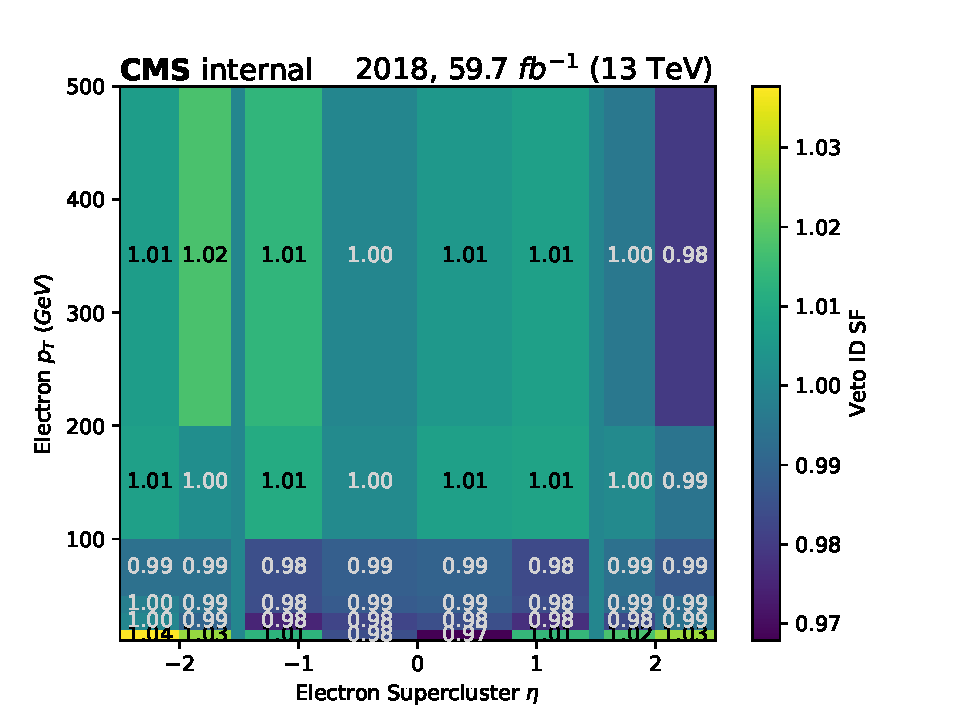
\includegraphics[width=0.45\textwidth]{ScaleFactors/Electron/electron_id_veto_2018.pdf}
    \caption{
      Scale factors for the identification efficiency of tight (left) and veto (right) electrons are shown for 2017 (top) and
      2018 (bottom). The scale factors are provided in bins of electron $\pt$ and $\eta$.
    }
    \label{fig:sf_electron_id}
  \end{center}
\end{figure}

\begin{figure}[ht!]
  \begin{center}
    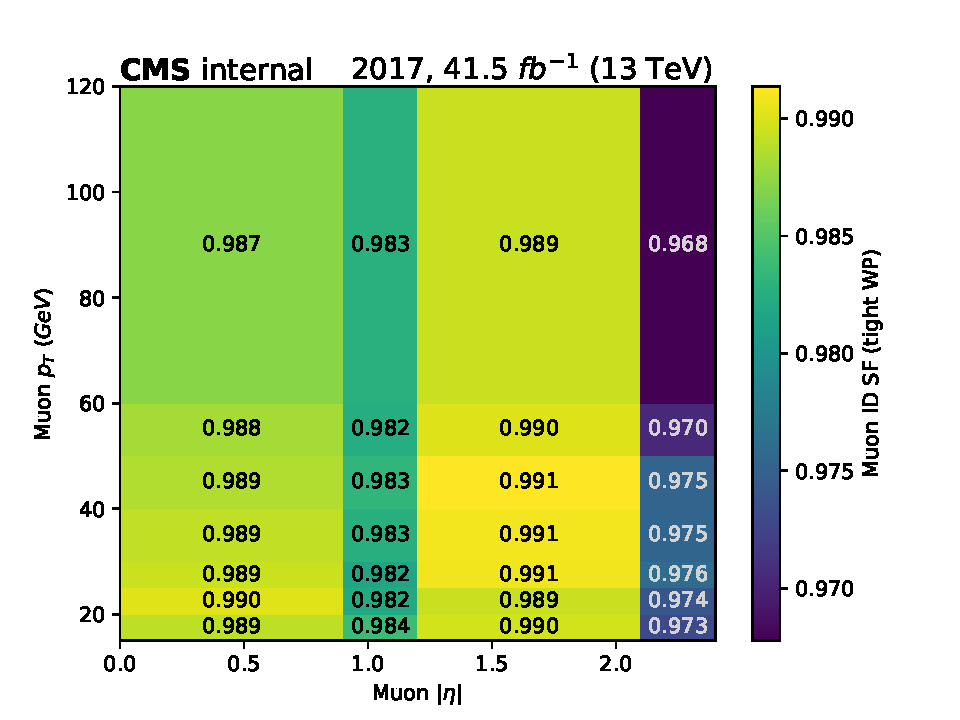
\includegraphics[width=0.49\textwidth]{ScaleFactors/Muon/NUM_TightID_DEN_TrackerMuons_abseta_pt_2017.pdf}
    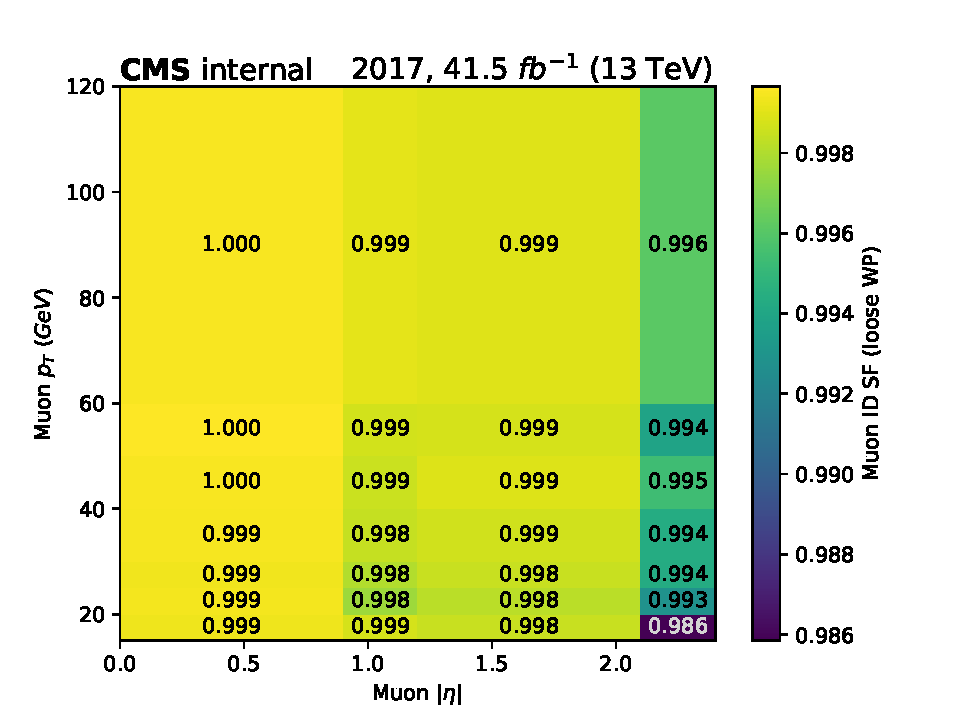
\includegraphics[width=0.49\textwidth]{ScaleFactors/Muon/NUM_LooseID_DEN_TrackerMuons_abseta_pt_2017.pdf} \\
    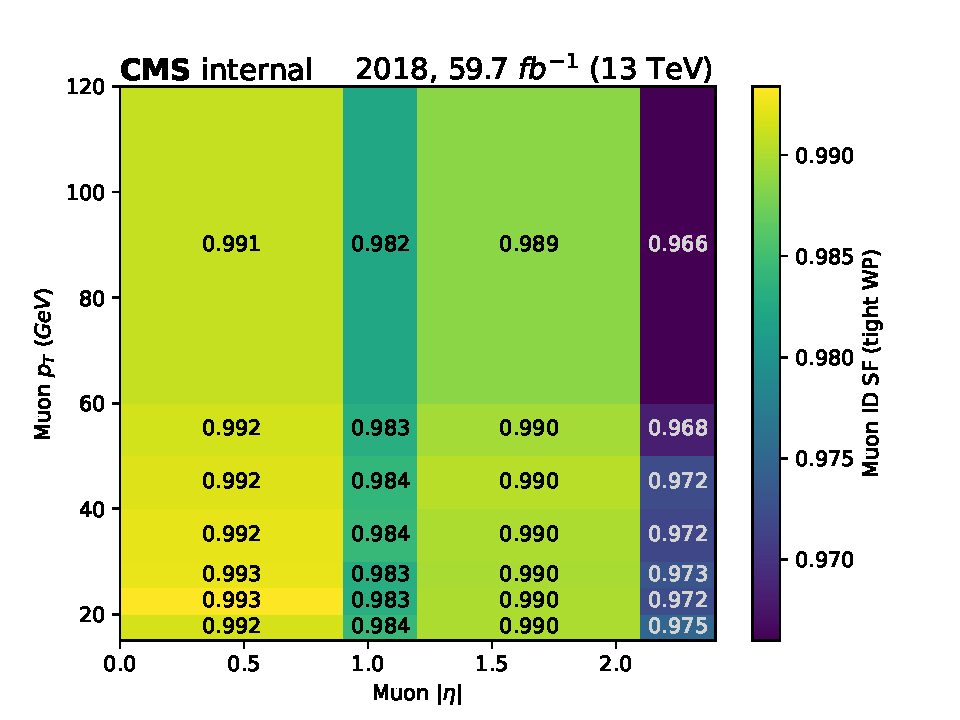
\includegraphics[width=0.49\textwidth]{ScaleFactors/Muon/NUM_TightID_DEN_TrackerMuons_abseta_pt_2018.pdf}
    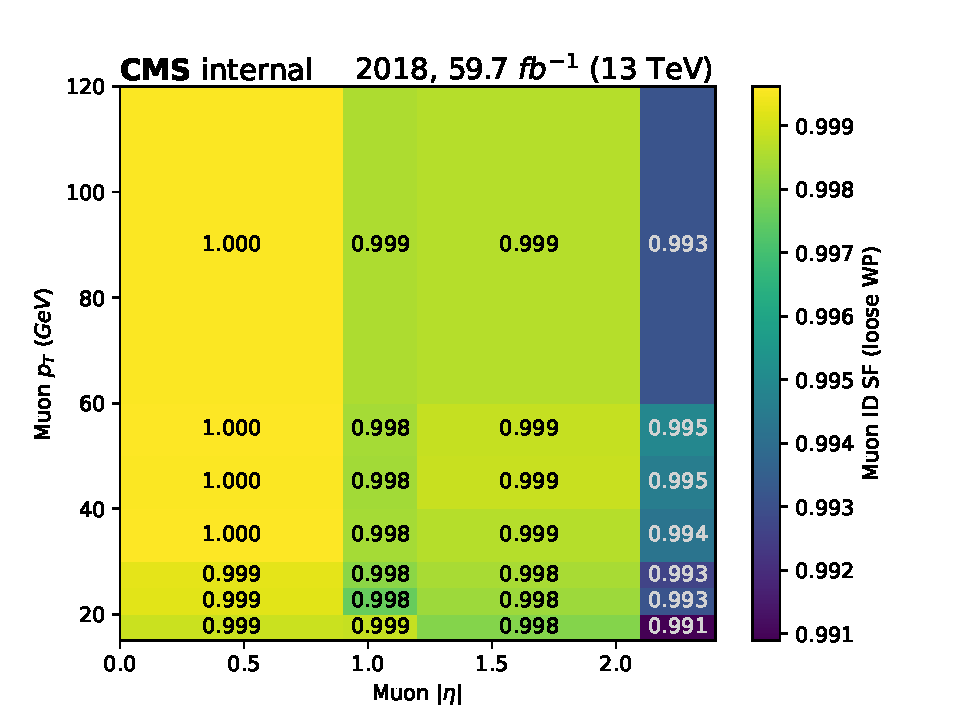
\includegraphics[width=0.49\textwidth]{ScaleFactors/Muon/NUM_LooseID_DEN_TrackerMuons_abseta_pt_2018.pdf}
    \caption{
      Scale factors for tight (left) and veto (right) muon identification are shown for 2017 (top) and
      2018 (bottom). The scale factors are provided in bins of muon $\pt$ and $\eta$.
    }
    \label{fig:sf_muon_id}
  \end{center}
\end{figure}

\begin{figure}[ht!]
    \begin{center}
        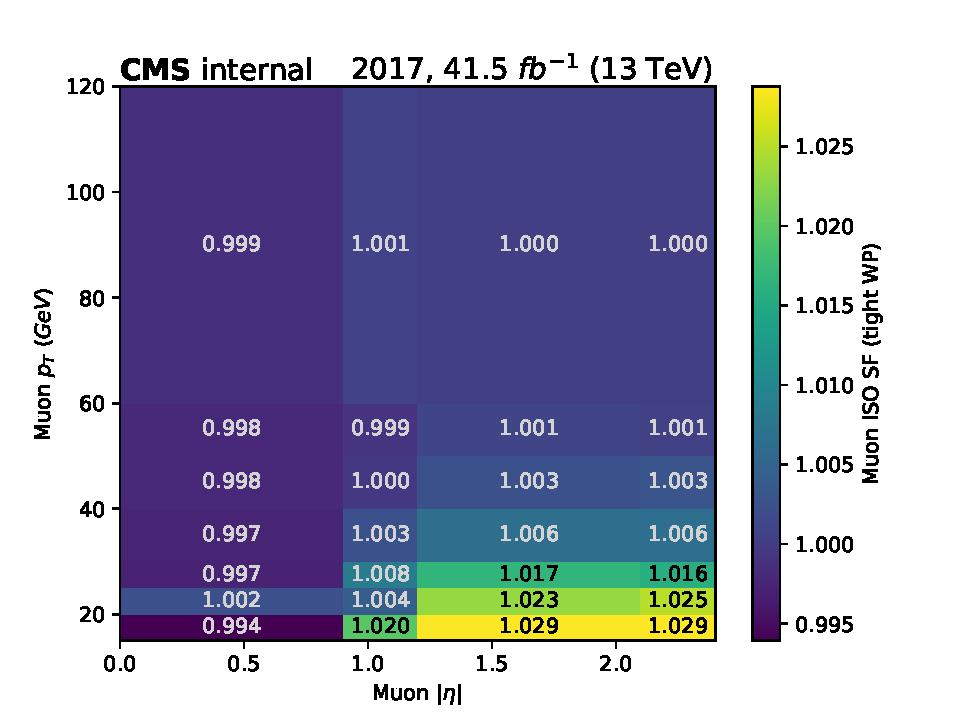
\includegraphics[width=0.49\textwidth]{ScaleFactors/Muon/NUM_TightRelIso_DEN_TightIDandIPCut_abseta_pt_2017.pdf}
        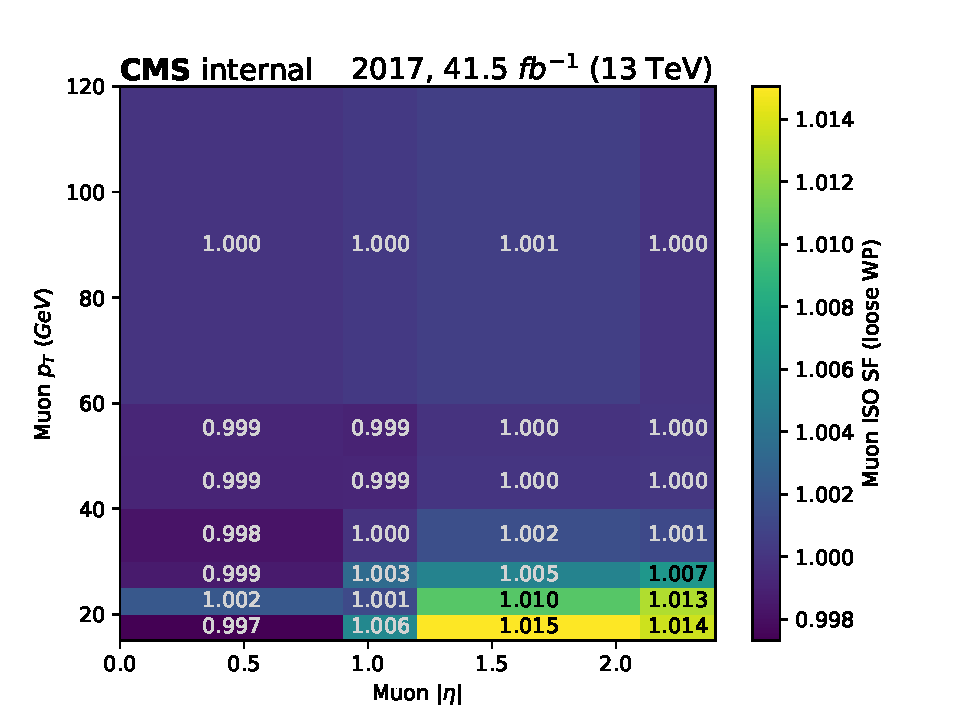
\includegraphics[width=0.49\textwidth]{ScaleFactors/Muon/NUM_LooseRelIso_DEN_LooseID_abseta_pt_2017.pdf} \\
        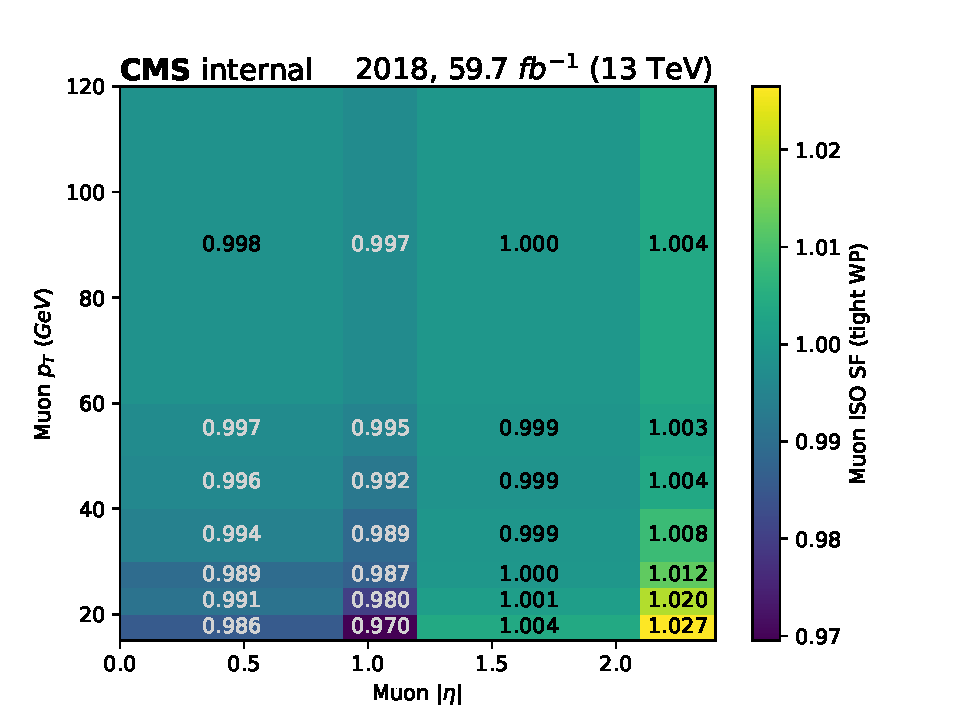
\includegraphics[width=0.49\textwidth]{ScaleFactors/Muon/NUM_TightRelIso_DEN_TightIDandIPCut_abseta_pt_2018.pdf}
        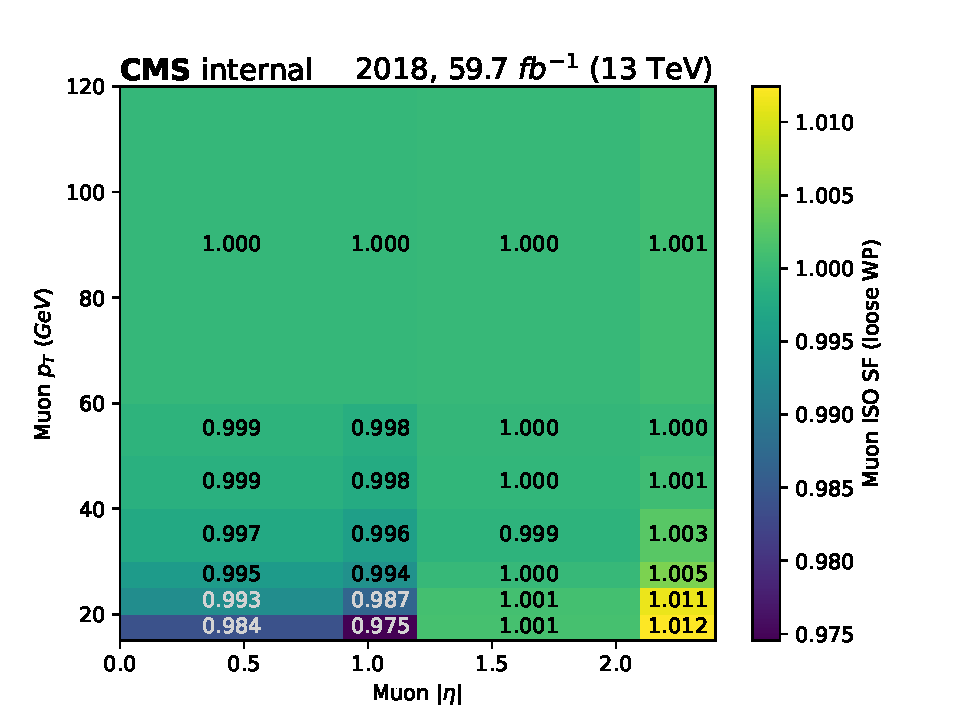
\includegraphics[width=0.49\textwidth]{ScaleFactors/Muon/NUM_LooseRelIso_DEN_LooseID_abseta_pt_2018.pdf}
        \caption{
            Scale factors for tight (left) and veto (right) muon isolation are shown for 2017 (top) and
            2018 (bottom). The scale factors are provided in bins of muon $\pt$ and $\eta$.
        }
      \label{fig:sf_muon_iso}
    \end{center}
\end{figure}

\clearpage

\subsection{Lepton veto efficiency reweighting}

To reduce contribution from $W(\ell \nu)+$ jet(s) events in the analysis signal region (SR), 
events are rejected if they contain any
identified charged lepton. However, due to finite efficiencies of the
reconstruction and identification of these candidates, $W(\ell \nu)+$ jet(s)
events still contribute significantly. Furthermore, the differences in veto efficiency between data and MC
need to be taken into account. For these purposes, the ``veto-weight'' method is used.
In this method, simulated events in the SR are allocated a veto weight instead of
being removed completely if they have charged lepton(s) in the final state. Such events with
identified leptons can enter the SR with a veto weight dependent on the identification, isolation and reconstruction 
efficiency scale factors for the identified objects
in the event. The veto weight $\omega$ is calculated as:

\begin{equation}
    \omega = \prod_{i \ \epsilon \ leptons} (1-SF_{i}) 
\end{equation}

where the product above runs over all identified veto leptons in the event (i.e. electrons, muons and taus).
$SF_{i}$ represents the total scale factor for the lepton $i$, which is the product of identification and isolation
scale factors as described in Sec.~\ref{subsec:lepton_id_reweighting}. It can be observed that this method is equivalent
to the ordinary method with hard-veto on events with leptons, as $SF \approx 1$ for events with well identified leptons,
making the event weight, $\omega \approx 0$, hence suppressing the contribution of the event in the SR.
Comparing the simulated event yields with hard
lepton veto applied (instead of lepton veto weights), it is observed that the lepton veto weights in the signal region
introduces a small correction $\ll 1\%$.

The uncertainty on these veto weights are computed by varying the veto weights within their uncertainties and
propagating the variation into the $\mjj$ distribution in the SR. Since the lepton kinematics are not largely
correlated with the kinematics of two outgoing VBF jets, the uncertainties are observed to be flat as a function
of $\mjj$.

% In Fig.~\ref{fig:sr_veto_weights}, the impact of the veto weight
% corrections (compared to the hard lepton veto) on the $\Wlvjets$ process in the VBF signal region, 
% and the uncertainty on the veto weights are shown. It can be observed that the correction
% coming from the veto weights is typically small ($\ll 1\%$), and the uncertainties on the veto weights are small
% and uncorrelated with the invariant mass of two VBF jets, $\mjj$.

% \begin{figure}[ht!]
%   \begin{center}
%     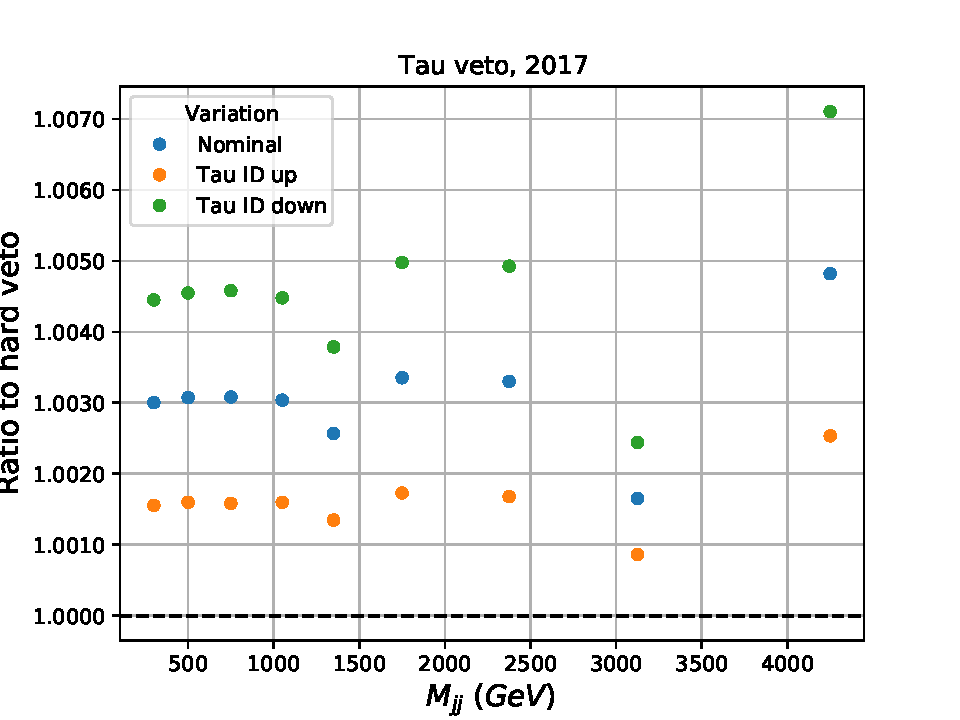
\includegraphics[width=0.45\textwidth]{ScaleFactors/VetoWeights/tau_vetow_variations_2017.pdf}
%     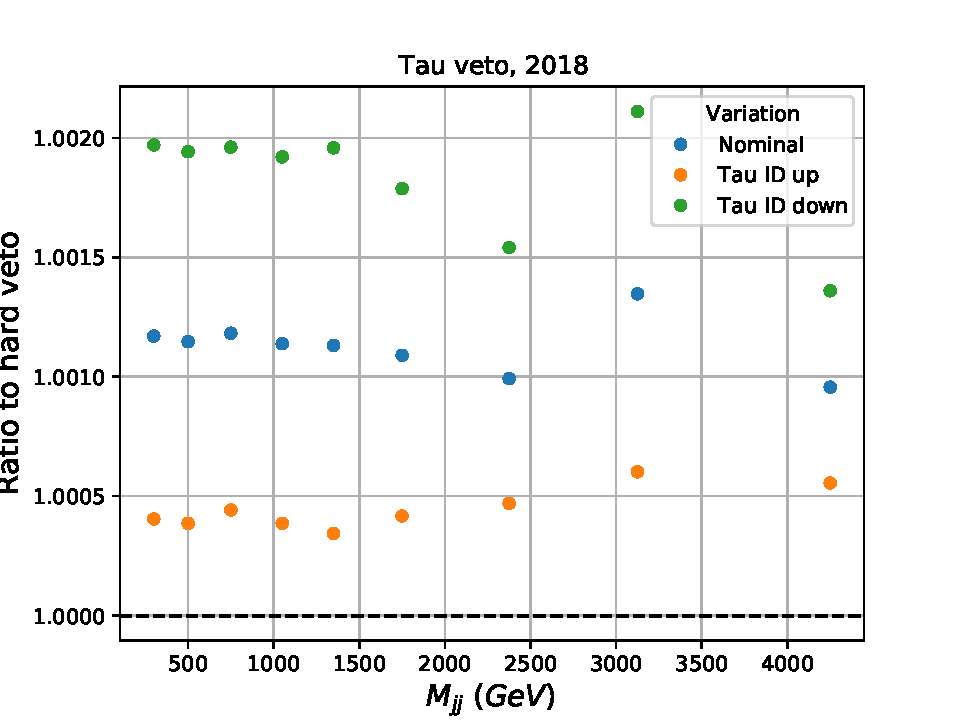
\includegraphics[width=0.45\textwidth]{ScaleFactors/VetoWeights/tau_vetow_variations_2018.pdf} \\
%     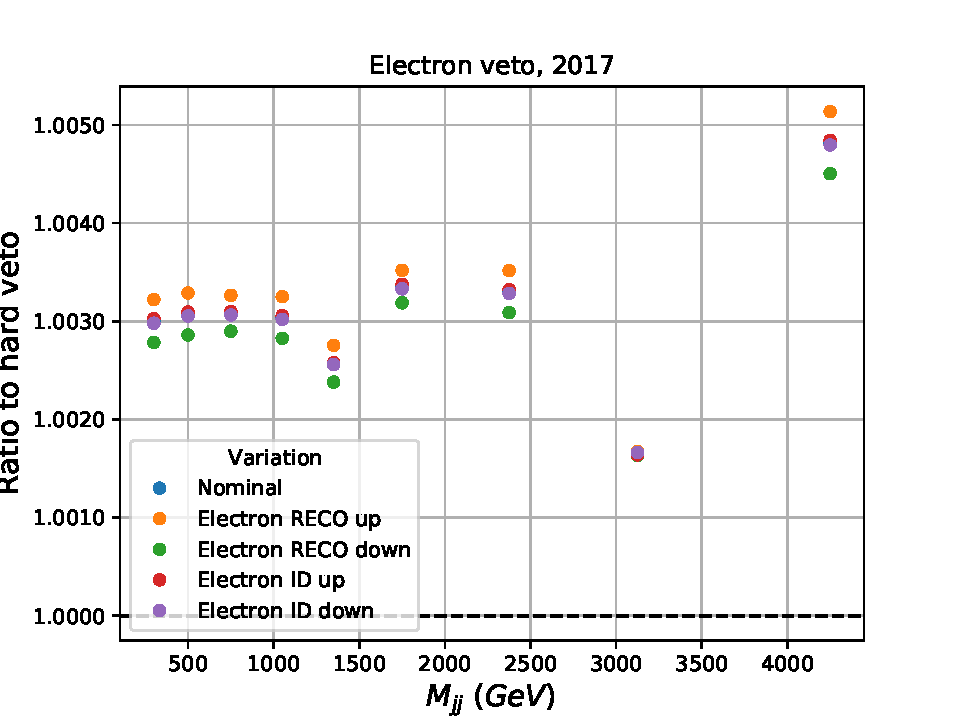
\includegraphics[width=0.45\textwidth]{ScaleFactors/VetoWeights/ele_vetow_variations_2017.pdf}
%     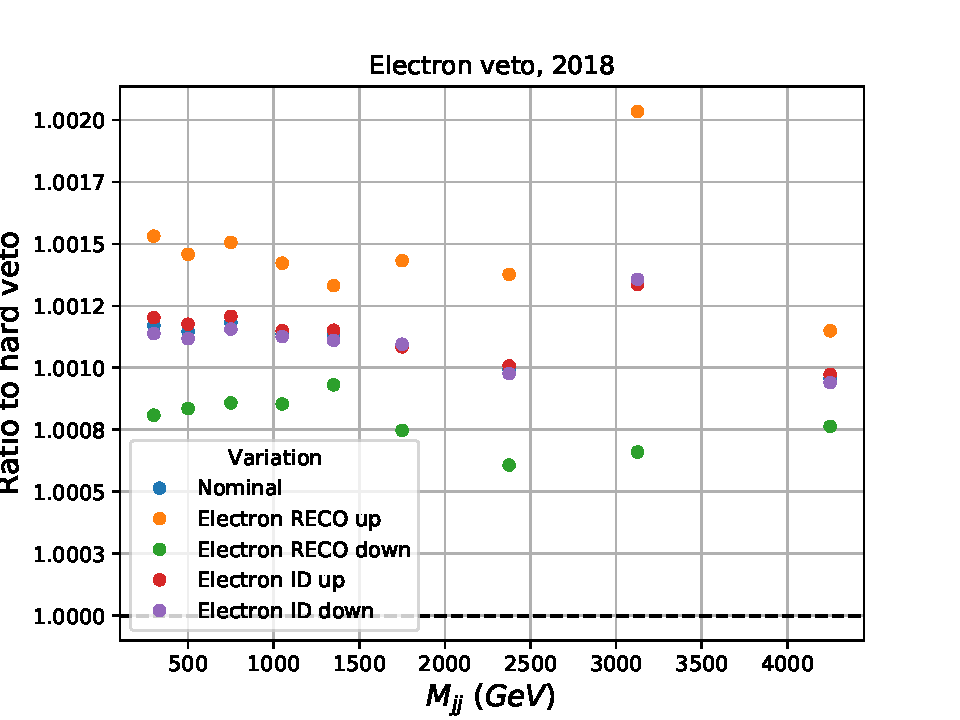
\includegraphics[width=0.45\textwidth]{ScaleFactors/VetoWeights/ele_vetow_variations_2018.pdf} \\
%     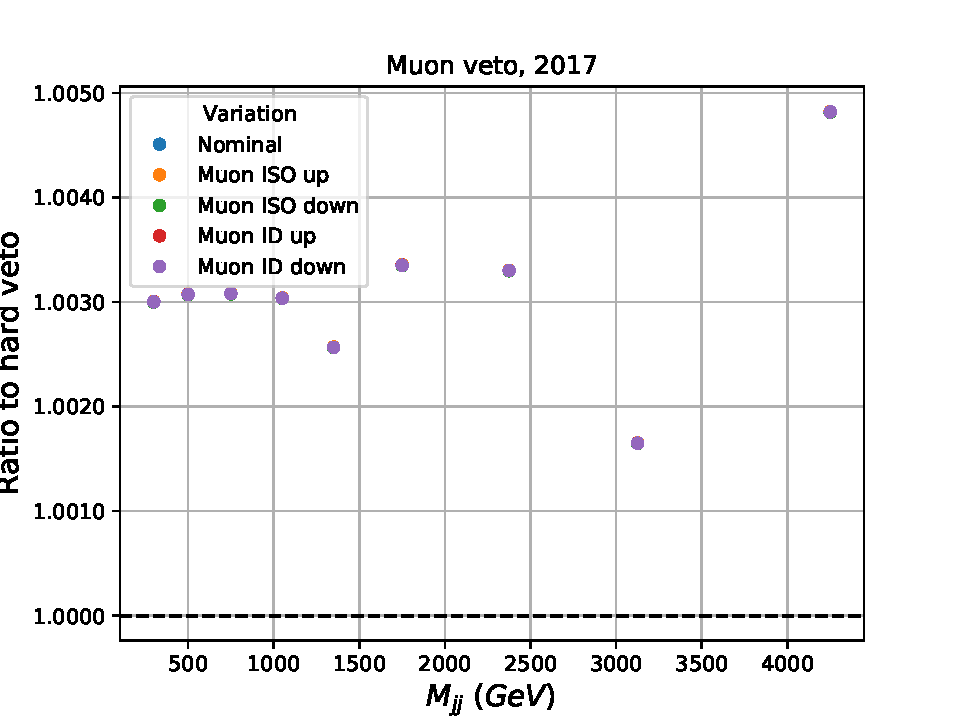
\includegraphics[width=0.45\textwidth]{ScaleFactors/VetoWeights/muon_vetow_variations_2017.pdf}
%     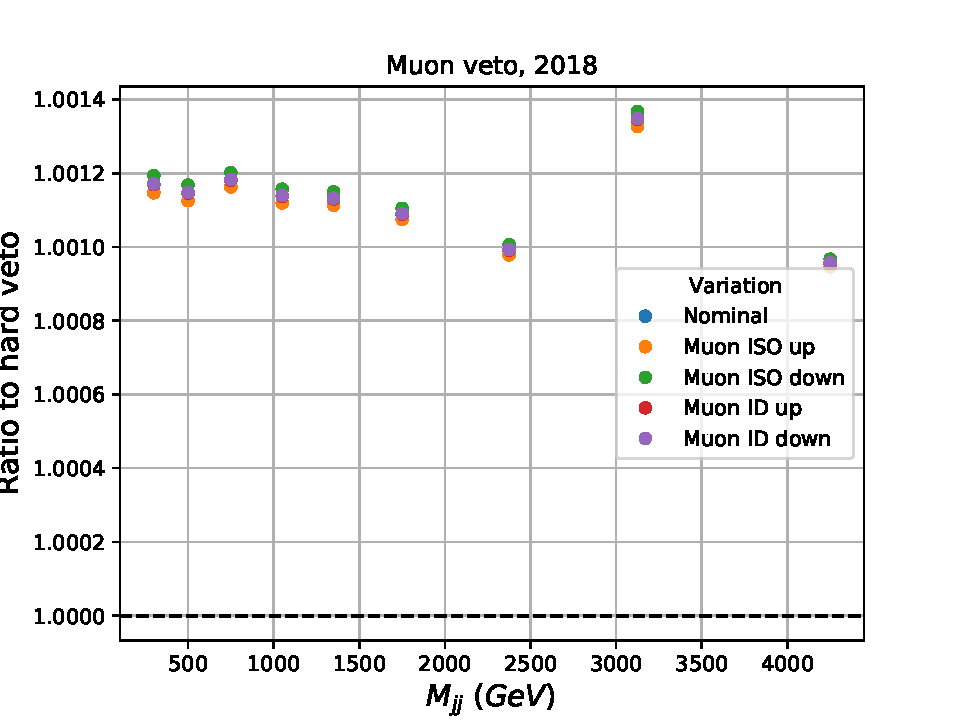
\includegraphics[width=0.45\textwidth]{ScaleFactors/VetoWeights/muon_vetow_variations_2018.pdf}
%     \caption{
%       The impact of the veto weight corrections on $\Wlvjets$ process in the signal region. The correction with the nominal
%       lepton veto weight and the uncertainties of the veto weight are shown, and the event yield ratio with the hard lepton veto
%       case is plotted. The top row corresponds to the tau veto, middle row to electron veto, and last row corresponds to
%       muon veto. Left and right columns represent 2017 and 2018 datasets, respectively. 
%     }
%     \label{fig:sr_veto_weights}
%   \end{center}
% \end{figure}

% \subsection{Efficiency reweighting for b-jet vetos}

% \emph{TODO: Fill this section.}

\subsection{Reweighting For HF Noise Cuts}
\label{subsec:hf_weighting}

As will be explained in Sec.~\ref{subsec:hfnoise}, several noise-cleaning cuts are implmented to reduce the contribution 
from mis-measured forward jets,
reconstructed in the Forward HCAL (HF) detector (i.e. $|\eta| > 3.0$). To account for the difference in the impact of these cuts in
data and MC, a per-jet scale factor is applied to the events in MC. These scale factors are derived by calculating the efficiency 
of these cuts on $\Zmmjets$ and $\gamma$ + jets events in data and MC, as a function of jet $\pt$ and $\eta$, and taking 
the ratio of those two efficiencies. 

The HF noise scale factors are applied for each HF jet in the event which would be taken into account for the HF cuts (i.e. $\pt > 100$ GeV 
and $\Delta\phi(j,\ptmiss) > 2.5$), as a function of $\pt$ and $\eta$ of the jet. The event weight is calculated by multiplying the individual jet weights:

\begin{equation}
    \omega_{event} = \prod_{jet \in HF} \omega_{jet} (\pt, \eta)
\end{equation}

where the product runs over each jet with $\pt > 100$ GeV and $\Delta\phi(j,\ptmiss) > 2.5$\footnote{These cuts are required
to be compatible with the application of HF cuts described in Sec.~\ref{subsec:hfnoise}. $\Delta\phi > 2.5$ requirement on
the jets being considered is utilized to pick jets that are reconstructed back-to-back (i.e. high $\Delta\phi$) with the missing
transverse momentum}.
The per-jet scale factors $\omega_{jet}$ are shown in Fig.~\ref{fig:hf_scale_factors} for 2017 and 2018, together with their statistical uncertainties. 
For the statistically limited phase space of very high $\pt$ and $\eta$ (where the scale factor is measured to be $0$), 
the scale factor in the closest $[ \pt, \eta ]$ bin is applied to the HF jet.

\begin{figure}[ht!]
    \begin{center}
        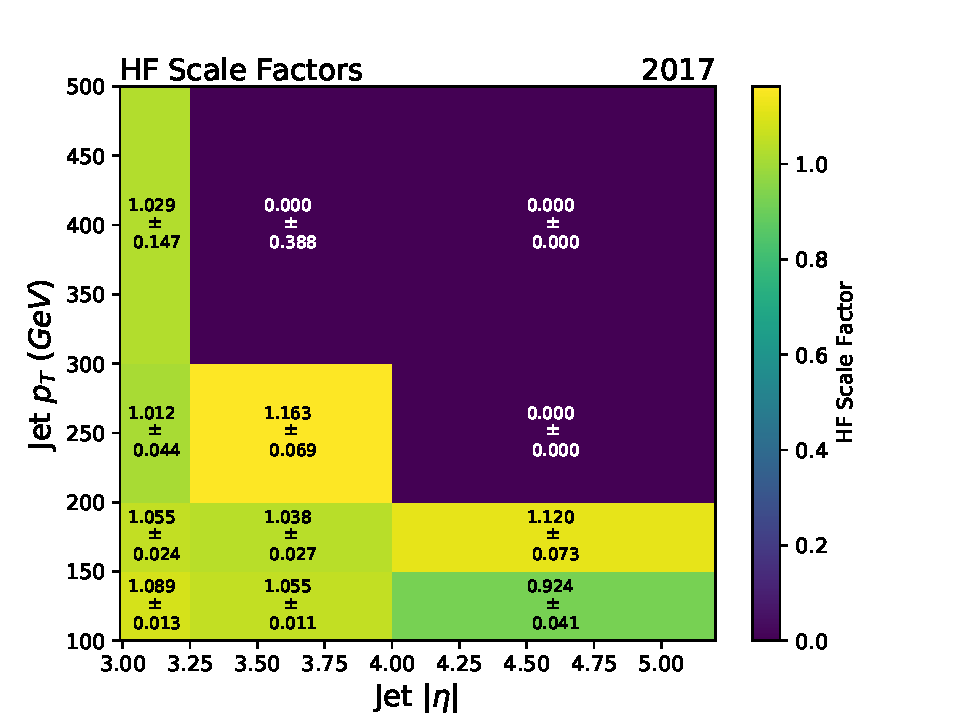
\includegraphics[width=0.49\textwidth]{ScaleFactors/HFCuts/hf_sf_2017.pdf}
        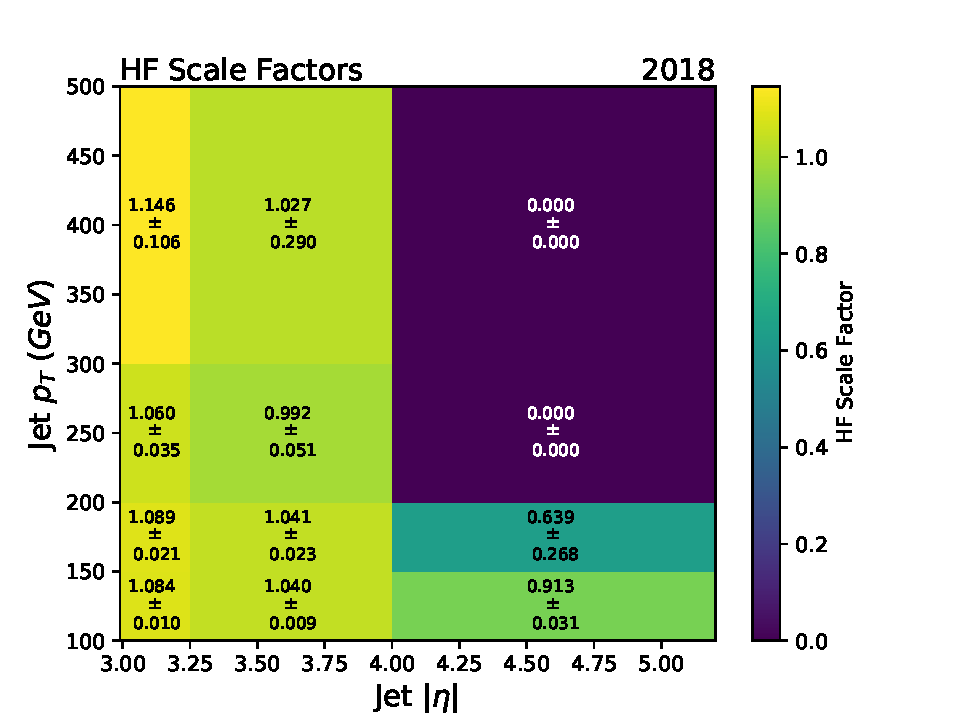
\includegraphics[width=0.49\textwidth]{ScaleFactors/HFCuts/hf_sf_2018.pdf}
        \caption{
            HF scale factors and their statistical uncertainties as a function of jet $\pt$ and $\eta$, for 2017 (left) and 2018 (right). 
            For the phase space with statistical limitations (i.e. $SF=0$), the scale factor in the closest $[ \pt, \eta ]$ bin is applied to the HF jet.
          }
        \label{fig:hf_scale_factors}
    \end{center}
\end{figure}

\clearpage

\subsection{Reweighting for ECAL pre-firing}
\label{subsec:prefiring_weighting}

Prefiring is a problem with the 2017 dataset that results from L1 trigger primitives
in the ECAL endcap being incorrectly assigned to an earlier bunch crossing because
of a timing issue. In most cases, the event to which the trigger primitives are now assigned to
fail to pass the HLT selection and is discarded. This makes the event for which the trigger
primitives were originally belonged to be discarded as well, which results in a loss of trigger
efficiency. A solution has been developed by parametrizing
the probability of a jet or photon in the event causing prefiring in terms of their
$\pt$ and $\eta$. In this analysis, the prefiring weights are applied based on the parametrization
provided by the JME POG \cite{CMS:PrefiringTwiki}, and a central implementation provided in the
NanoAOD-tools software is used \cite{CMS:PrefiringNanoAODTools}. In this implementation, a per-event
prefiring weight is computed as:

\begin{equation}
    \omega = 1 - P(prefiring) = \prod_{i=photons,jets} (1 - \epsilon_{i}^{pref}(\pt, \eta))
\end{equation}

where $\epsilon_{i}^{pref}$ is the prefiring probability caused by a single photon or a jet, and the product
runs over the photons and jets reconstructed in the event.
The $\mjj$ distributions with the nominal prefiring weight applied to simulation, together with the
up and down variations of the prefiring weight are shown in Figs.~\ref{fig:prefiring_1} and \ref{fig:prefiring_2}.
It can be observed that the uncertainty due to the prefiring weight increases with higher $\mjj$. 

\begin{figure}[htbp]
  \centering
    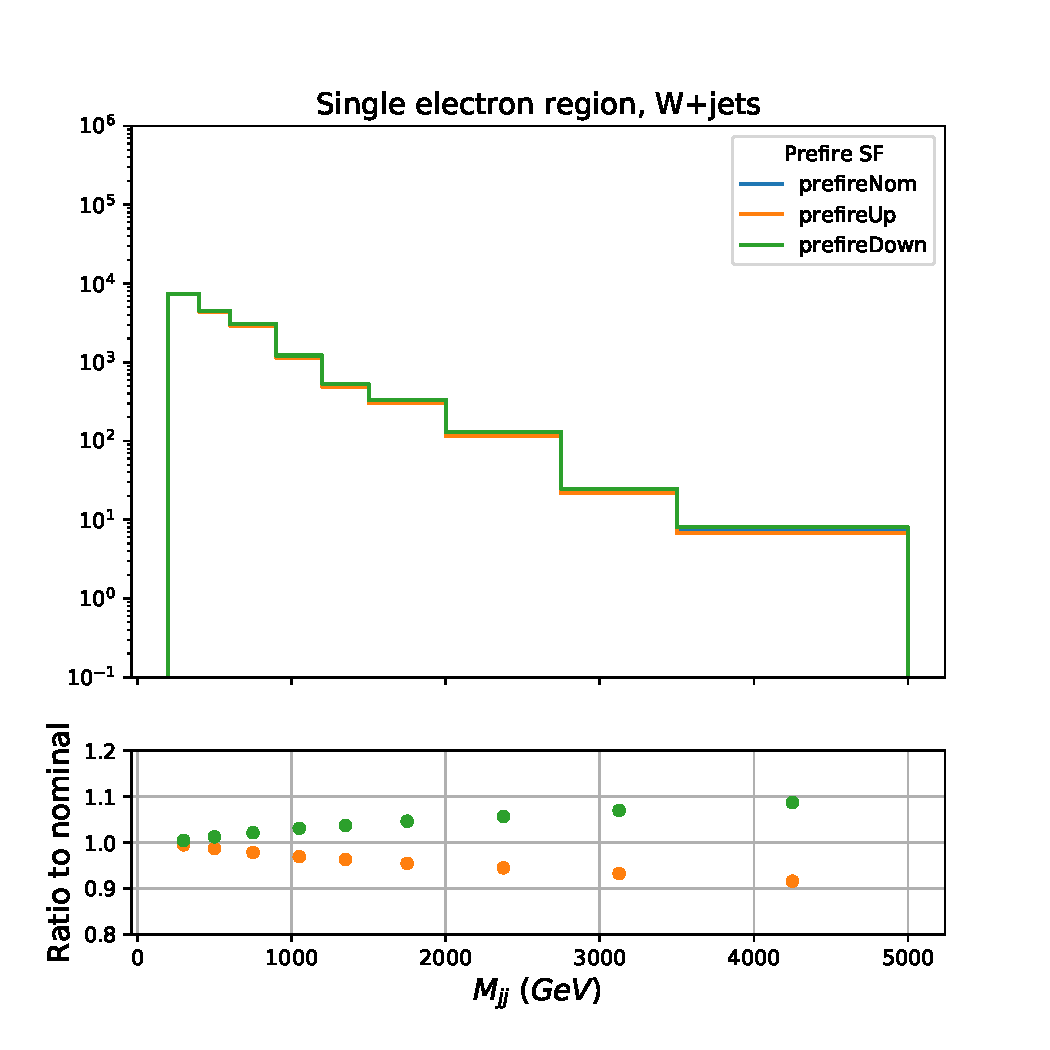
\includegraphics[width=0.49\textwidth]{ScaleFactors/Prefire/cr_1e_vbf.pdf}
    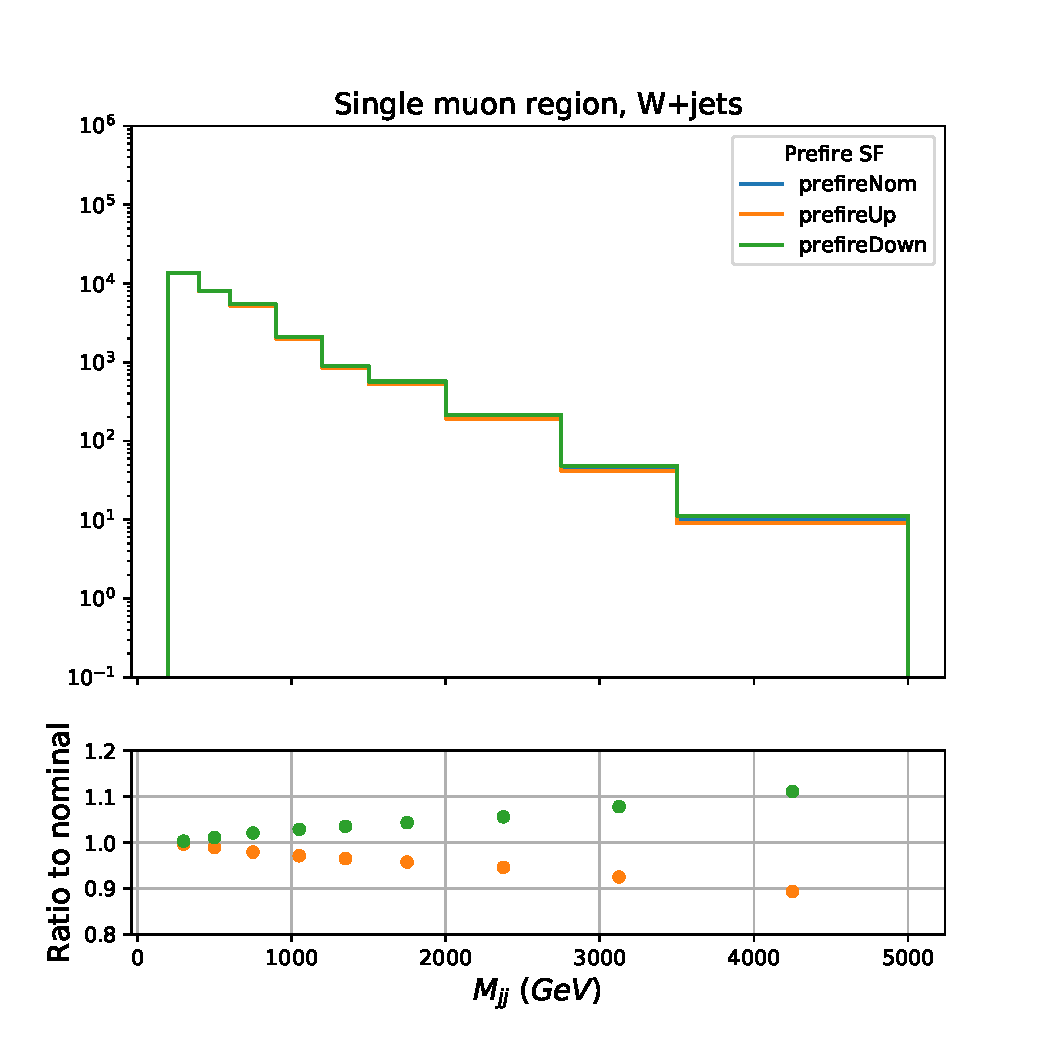
\includegraphics[width=0.49\textwidth]{ScaleFactors/Prefire/cr_1m_vbf.pdf} \\
    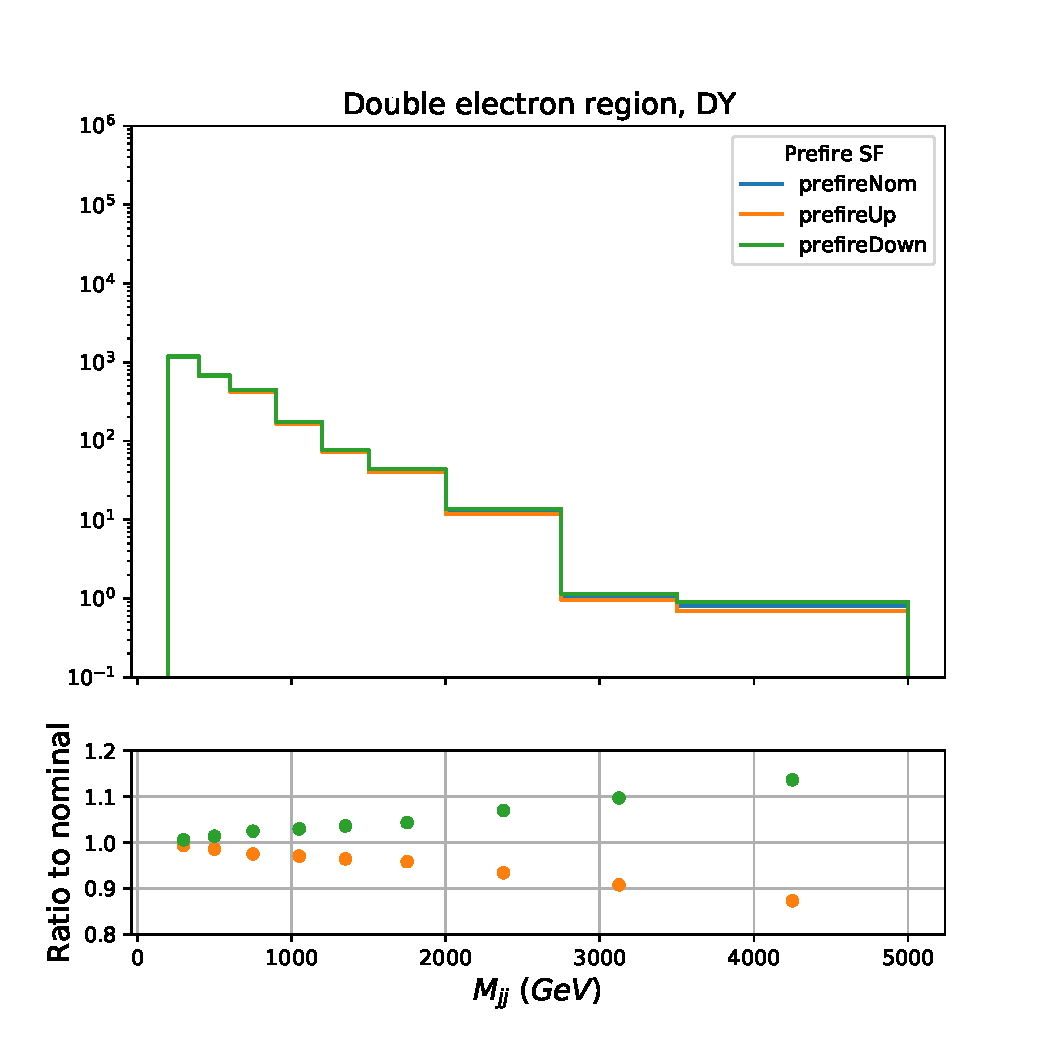
\includegraphics[width=0.49\textwidth]{ScaleFactors/Prefire/cr_2e_vbf.pdf}
    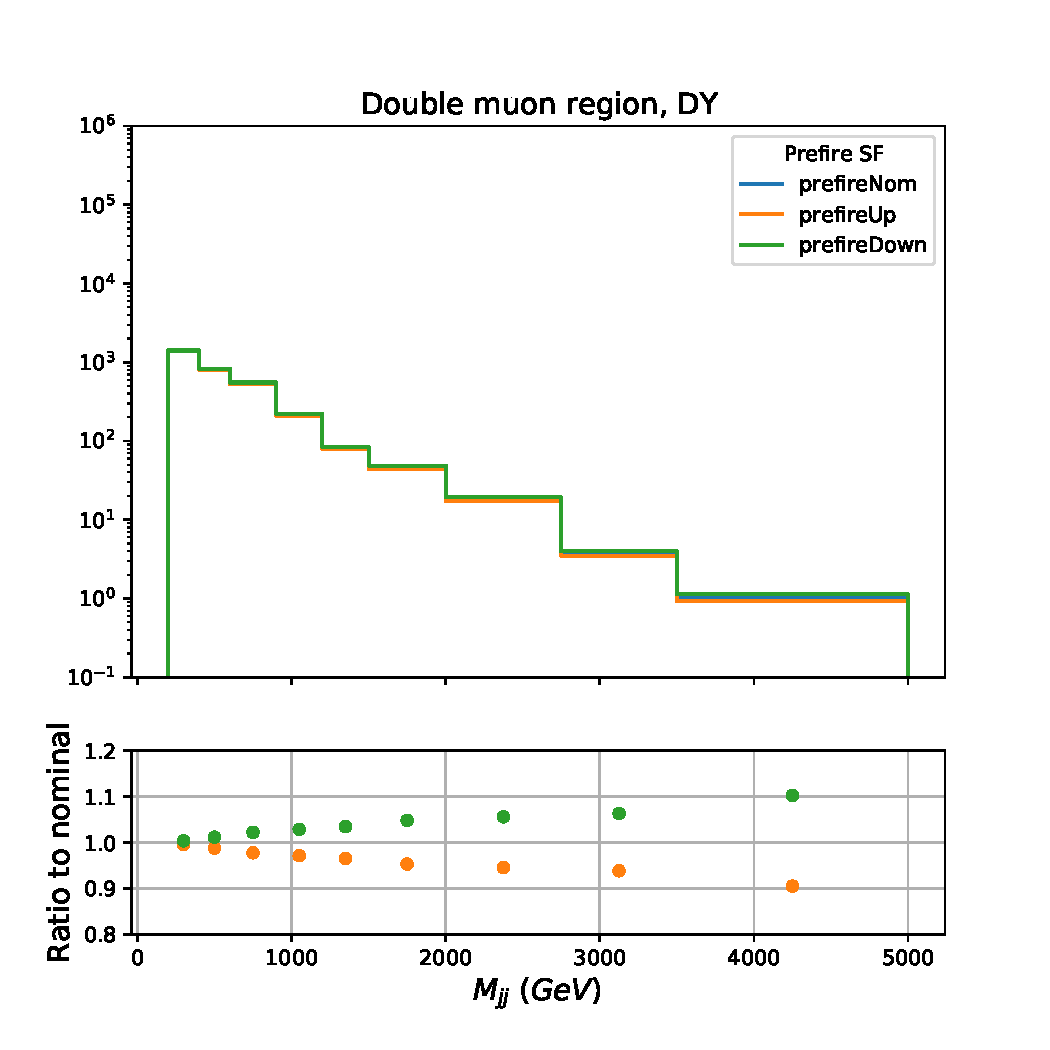
\includegraphics[width=0.49\textwidth]{ScaleFactors/Prefire/cr_2m_vbf.pdf}
    \caption{The $\mjj$ distributions with the nominal prefiring weights and its variations
    are shown for $\Wjets$ simulation in single lepton CRs (top), and $\Zjets$ simulation in
    double lepton CRs (bottom).}
    \label{fig:prefiring_1}
\end{figure}

\begin{figure}[htbp]
  \centering
    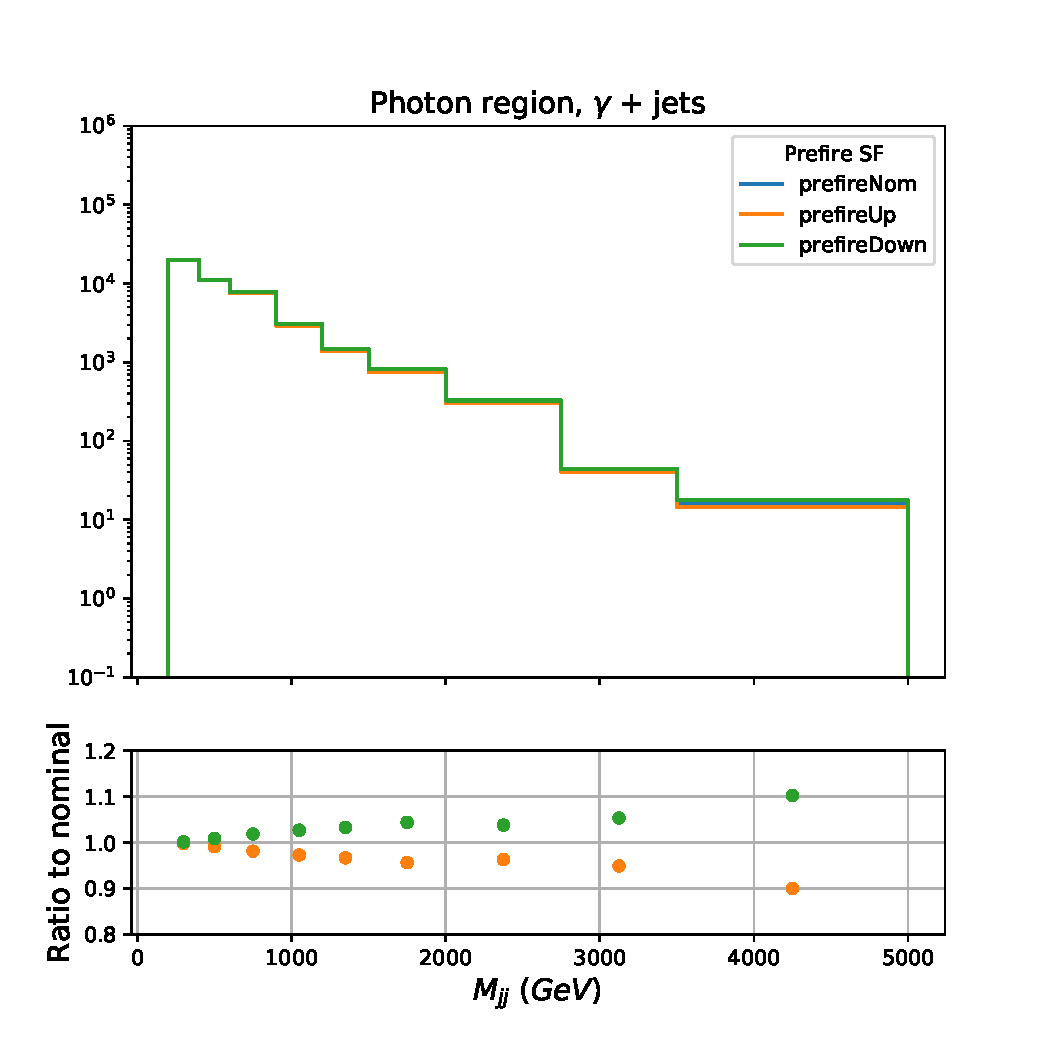
\includegraphics[width=0.49\textwidth]{ScaleFactors/Prefire/cr_g_vbf.pdf}
    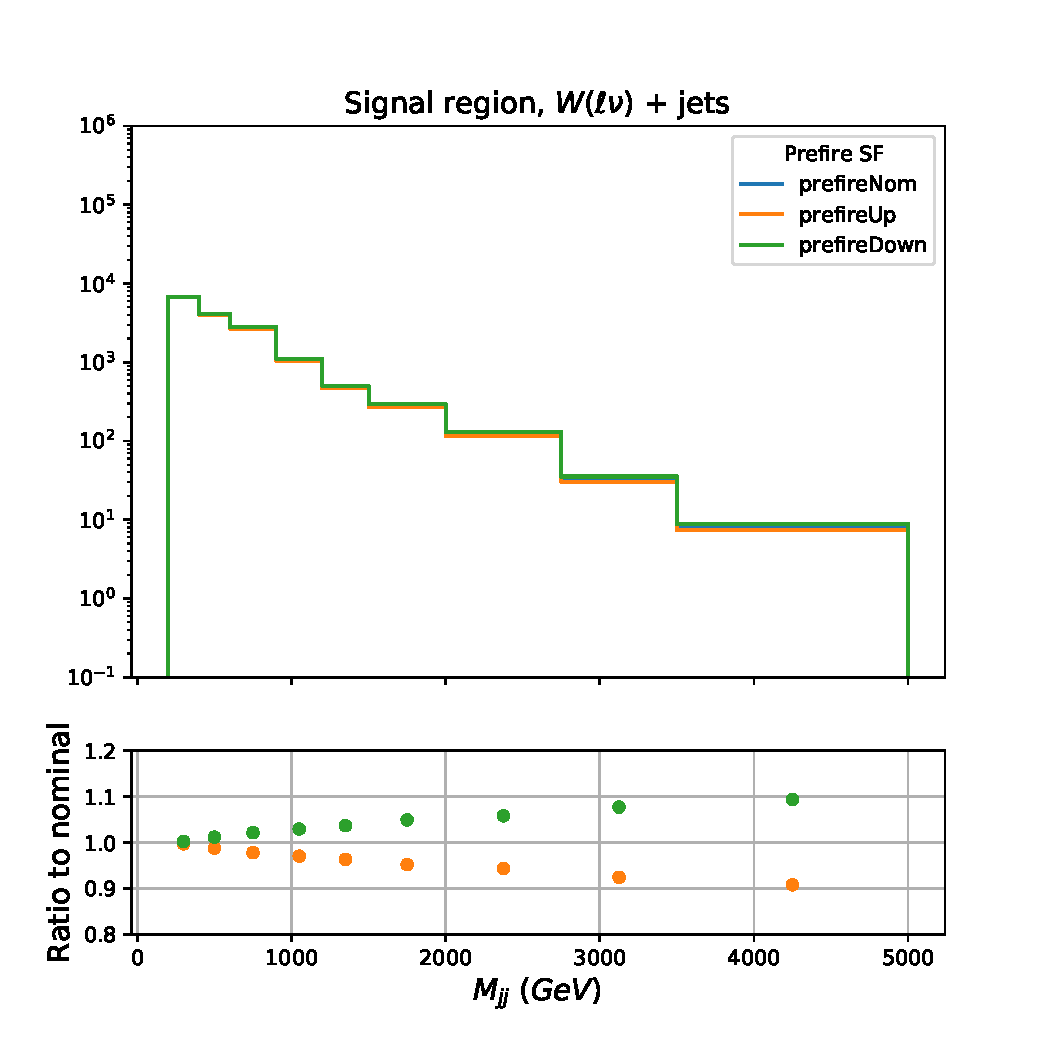
\includegraphics[width=0.49\textwidth]{ScaleFactors/Prefire/sr_vbf_qcd_wlv.pdf} \\
    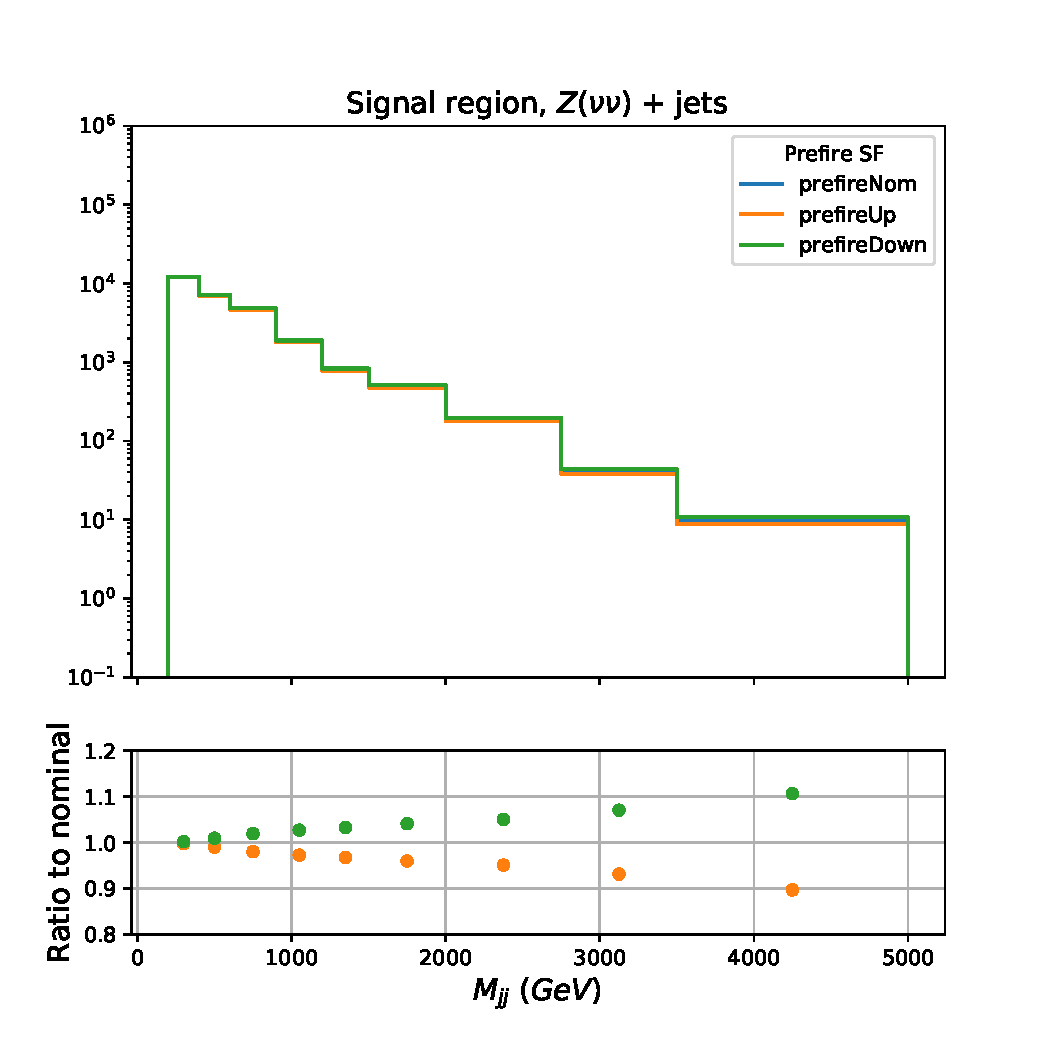
\includegraphics[width=0.49\textwidth]{ScaleFactors/Prefire/sr_vbf_qcd_zvv.pdf}
    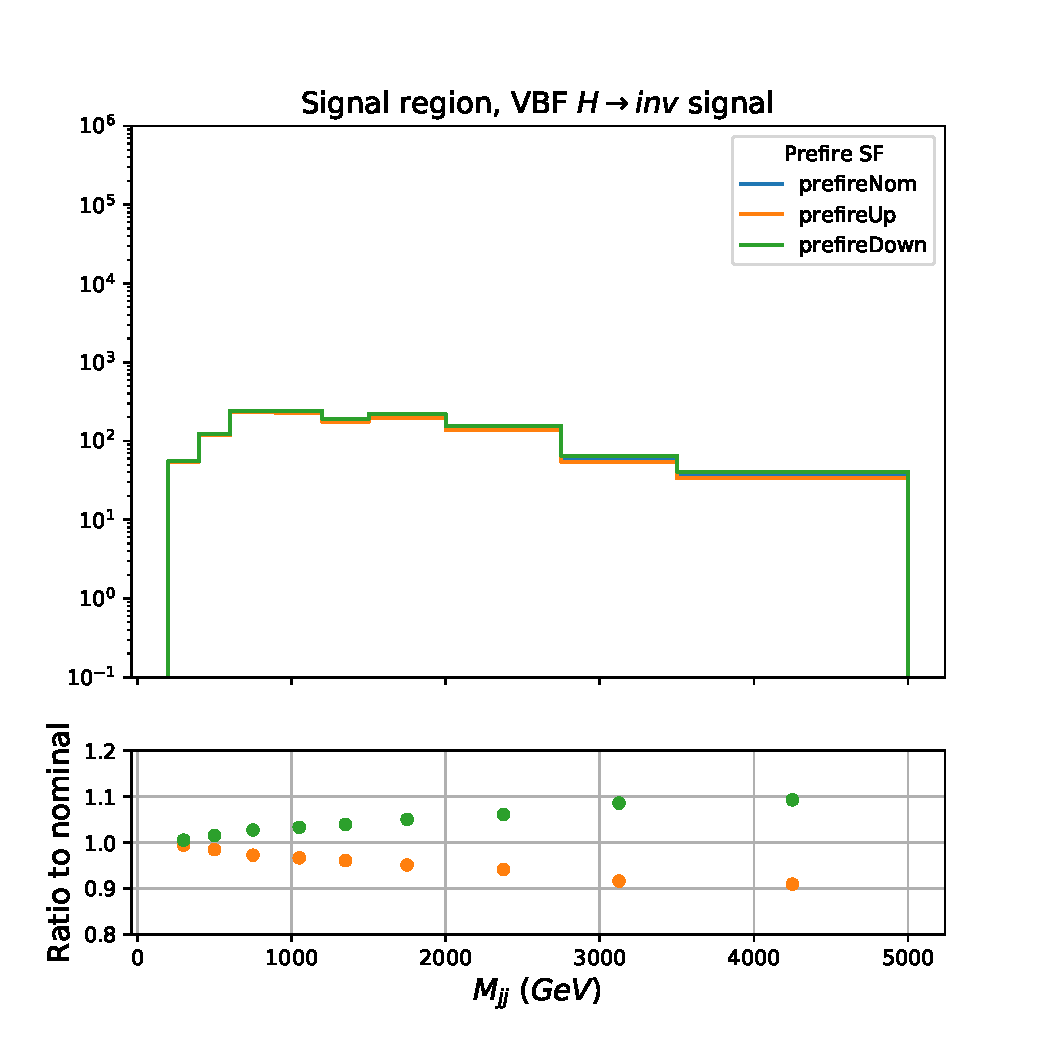
\includegraphics[width=0.49\textwidth]{ScaleFactors/Prefire/sr_vbf_vbfhinv.pdf}
    \caption{The $\mjj$ distributions with the nominal prefiring weights and its variations
    are shown for $\gamma$ + jets simulation in the photon CR (top left), $W(\ell\nu)$ + jets (top right),
    $Z(\nu\nu)$ + jets (bottom left) and VBF $\hinv$ (bottom right) in the signal region.}
    \label{fig:prefiring_2}
\end{figure}

\subsection{Higher-order reweighting}
\label{sec:nlo}

As will be detailed in Sec.~\ref{subsec:likelihood_fit}, this analysis uses the ratios of $\Vjets$ distributions in signal and control regions 
to constrain the final background estimate for $\Zvvjets$ and $\Wlvjets$ processes. 
As signal and control regions both have large statistical power, precise predictions of these ratios are necessary. 
To achieve this goal, next-to-leading-order (NLO) in QCD simulation samples are used for $\Wlvjets$ and $\Zlljets$ backgrounds, 
and corrected with higher-order EWK corrections. 
To model the $\gamma$ + jets background in photon control region, leading-order (LO) in QCD simulation samples are used instead,
which are then reweighted using higher-order QCD and EWK corrections. 
These corrections are described in more detail in the following subsections. A concise overview of which corrections are applied to 
which processes is given in Tab.~\ref{tab:higher_order_summary}.

\begin{table}[ht!]
    \centering
    \small
    \def\arraystretch{1.5}
    \caption{Summary of higher-order corrections applied to simulated samples. For each boson production process, 
      separate samples and corrections are available for the EWK and QCD production modes. ``MC order'' reflects the 
      perturbative order used in the generation of the simulation sample, while the further columns represent corrections 
      applied on a per-event level in the analysis process.}
    \begin{tabular}{c c c c c c}
        \textbf{Boson} & \textbf{Production mode}  & \textbf{MC order} & \textbf{NLO QCD}  & \textbf{NLO EWK} \\\hline\hline
    \multirow{2}{*}{Z} & QCD & NLO & --         & \checkmark \\
                       & EWK & LO  & \checkmark & -- \\\hline
    \multirow{2}{*}{W} & QCD & NLO & --         & \checkmark \\
                       & EWK & LO & \checkmark & -- \\\hline
    \multirow{2}{*}{$\gamma$} & QCD & LO &  \checkmark & \checkmark \\
    & EWK & LO & -- & -- \\\hline\hline

    \end{tabular}

    \label{tab:higher_order_summary}
\end{table}

\subsubsection{Generator-level boson construction}
All theory-based corrections of the $\Wlvjets$, $\Zlljets$, and $\gamma$ + jets backgrounds are parametrized as a function of the 
generator-level transverse momentum of the respective boson, $\ptv$. For $\Wlvjets$ and $\Zlljets$ events, this quantity is calculated as follows:

\begin{enumerate}
  \item If a boson is found in generator-level collection with \texttt{status = 62}, it's $\ptv$ is taken as the generator level $\ptv$.
  (If multiple such entries are found, highest $\ptv$ is chosen.)
  \item In the rare cases where the boson is not found in the generator-level collection, then the boson is defined as the four-vector sum of the selected leptons.
  Leptons are selected as described in the next two steps:
  % \item If there are dressed electrons or muons (taken from the \texttt{GenDressedLepton} collection) that are not coming from a tau decay, these leptons are selected
  % to compute $\ptv$.
  % \item If the dressed electrons or muons are found to be coming from a tau decay, or if there are no dressed leptons in the event, the generator-level taus 
  % are chosen to compute $\ptv$.
  \item If there are electrons or muons that are not coming from a tau decay, these leptons are selected to compute $\ptv$.
  \item If the electrons or muons are found to be coming from a tau decay, or if there are no leptons in the event, the generator-level taus 
  are chosen to compute $\ptv$.
\end{enumerate}

For $\gamma$ + jets events, the photon at generator-level is selected by requiring the following:
\begin{itemize}
    \item Photon needs to have \textit{status = 1}, indicating that it is a final state particle (i.e. a particle that is not decayed further by the generator). 
    \item Photon needs to have a prompt status flag. 
    \item $|\eta|<1.46$, so that the photon is in the barrel region. 
\end{itemize}

If there are multiple such photons, the one with highest $\pt$ is selected.

\subsubsection{Photon scale factors}

The photon scale factors are derived with a two-dimensional dependence on generator-level $\ptv$ and $\mjj$, and are shown for the MTR category in 
Fig.~\ref{fig:theory_sf_qcd_nlo_2d-photon}. These scale factors are applied to $\gamma$ + jets events as a NLO correction, and the correction depends
on the kinematics of the event.

\begin{figure}[ht!]
    \begin{center}
        \includegraphics[width=0.49\textwidth]{ScaleFactors/NLO/2d_gjets_gen_vpt_vbf_stat1.pdf}
        \caption{
            LO-to-NLO theory scale factors binned in the generator-level boson $\pt$ and $\mjj$, shown photon production.
            The k factors are derived within the generator-level VBF selection described in the text.
            The uncertainties quoted in each bin are the statistical uncertainties due to the finite size of the simulated samples.
          }
      \label{fig:theory_sf_qcd_nlo_2d-photon}
    \end{center}
\end{figure}

\subsubsection{EWK NLO corrections to QCD V processes}

Scale factors corresponding to NLO EWK corrections are obtained from Ref.~\cite{DMTheory} and applied as a function of the generator-level boson $\pt$
to each event. The scale factors are shown in Fig.~\ref{fig:theory_sf_ew_nlo}.

\begin{figure}[ht!]
    \begin{center}
        \includegraphics[width=0.49\textwidth]{ScaleFactors/NLO/nlo_ewk.pdf}
        \caption{
            EWK NLO scale factors for DY, W and photon production as a function of \ptv.
          }
      \label{fig:theory_sf_ew_nlo}
    \end{center}
\end{figure}

\subsubsection{QCD NLO corrections to EWK V processes}

The QCD NLO corrections to VBF $\Wjets$ and $\Zjets$ production have been calculated in Ref.~\cite{AN-2017-267} using the VBF@NLO program. 
They are parametrized in $\ptv$ and $\mjj$ and are shown in Fig.~\ref{fig:theory_sf_qcd_nlo_for_ewk}.

\begin{figure}[ht!]
    \begin{center}
        \includegraphics[width=0.49\textwidth]{ScaleFactors/NLO/nlo_qcd_for_ewk_dy.pdf}
        \includegraphics[width=0.49\textwidth]{ScaleFactors/NLO/nlo_qcd_for_ewk_w.pdf}
        \caption{
            QCD NLO scale factors for EWK DY, W production of $\ptv$ and $\mjj$.
          }
      \label{fig:theory_sf_qcd_nlo_for_ewk}
    \end{center}
\end{figure}

\clearpage

\subsubsection{NLO EWK Corrections on VBF Signal}
\label{subsubsec:vbf_nlo_ewk}

Next to leading order (NLO) EWK corrections on VBF signal are computed using the HAWK generator~\cite{HAWKGenerator}. 
The NLO corrections are computed in the VBF phase space, where events are selected based on the kinematics of the two final state VBF jets.
These kinematic selections are described in Sec.~\ref{sec:event_selection}.
The correction is calculated as a function of the $\pt$ of the Higgs boson, and is parametrized using the following fit function:

\begin{equation}
    \epsilon_{EWK}(p_T^{H}) = (1 - 0.000372 * p_T^{H} - 0.0304) / 0.95
\end{equation}

For each event in the VBF signal sample, this correction is applied based on the $\pt$ of the Higgs boson found in the generator-level collection.